% ============================================================
%  SISTEMA DE ALERTA TEMPRANA (SAT) — IIND-2104
%  Documento de Tesis — Versión Revisada
%  Autores: Nicolás Torres Pulido, Isabella Delgadillo Calero
%  Director: Juan Fernando Pérez Bernal
%  Citación: IEEE
% ============================================================

\documentclass[12pt, letterpaper, openany]{report}

\usepackage[utf8]{inputenc}
\usepackage[T1]{fontenc}
\usepackage[spanish]{babel}
\usepackage{amsmath, amssymb}
\usepackage{geometry}
\usepackage{setspace}
\usepackage{booktabs}
\usepackage{multirow}
\usepackage{array}
\usepackage{graphicx}
\usepackage{subcaption}
\usepackage{xcolor}
\usepackage{cite}
\usepackage[hidelinks]{hyperref}
\usepackage{url}
\usepackage{placeins}
\usepackage{longtable}
\usepackage{xcolor}
\usepackage{tabularx}

% Comando para espacios pendientes de completar por el autor
\newcommand{\TODO}[1]{\colorbox{yellow}{\textbf{[COMPLETAR: #1]}}}

\geometry{top=2.5cm, bottom=2.5cm, left=3cm, right=2.5cm}
\onehalfspacing
\renewcommand{\bibname}{Referencias}
% Usar "Tabla" consistentemente en todo el documento
\renewcommand{\tablename}{Tabla}
\renewcommand{\figurename}{Figura}
\graphicspath{{./}{figures/}{figuras/}}

% ============================================================
\begin{document}
% ============================================================

% ------------------------------------------------------------
%  PORTADA
% ------------------------------------------------------------
\begin{titlepage}
  \centering

  {\normalsize Universidad de los Andes\par}
  {\normalsize Facultad de Ingeniería\par}
  {\normalsize Departamento de Ingeniería Industrial\par}

  \vspace{1.5cm}
  \noindent\rule{\textwidth}{0.4pt}
  \vspace{0.5cm}

  {\LARGE Sistema de Alerta Temprana basado en \textit{Machine Learning}
  para la Predicción del Rendimiento Académico en IIND-2104
  Modelos Probabilísticos\par}

  \vspace{0.5cm}
  \noindent\rule{\textwidth}{0.4pt}

  \vspace{2cm}

  {\normalsize Nicolás Torres Pulido\par}
  {\normalsize Isabella Delgadillo Calero\par}

  \vspace{2cm}

  {\small \textit{Trabajo de grado presentado para optar por el título
  de Ingenieros Industriales en la Universidad de los Andes.}\par}

  \vspace{2cm}

  {\small Asesor: Ph.D. Juan Fernando Pérez Bernal\par}

  \vfill

  {\normalsize Bogotá D.C., Colombia, 2026\par}

\end{titlepage}

% ------------------------------------------------------------
%  ABSTRACT
% ------------------------------------------------------------
\chapter*{Resumen}
\addcontentsline{toc}{chapter}{Resumen}

El curso IIND-2104 Modelos Probabilísticos de la Universidad de los Andes 
presenta tasas históricas de reprobación superiores al 20\,\%. Hoy, el  profesor identifica estudiantes en dificultad cuando los problemas ya son visibles, en una etapa del semestre en que el margen de acción es 
reducido. Este trabajo diseña e implementa un Sistema de Alerta Temprana (SAT) basado en machine learning que predice con suficiente anticipación qué estudiantes están en riesgo de reprobar, dejando tiempo real para intervenir.


El sistema opera en dos momentos clave del semestre: la semana~6, 
tras el primer parcial (CP1), y la semana~11, tras el segundo (CP2), 
dejando ventanas de intervención amplias en ambos casos. Los datos 
integran cinco cohortes consecutivas del curso (202320-202520, 764 registros brutos), combinando calificaciones académicas y métricas de interacción con la plataforma Bloque Neón. Tras la depuración, el conjunto de modelado cuenta con 502 estudiantes activos.

Se evaluaron 148 configuraciones combinando cuatro algoritmos de 
clasificación (Regresión Logística, Árbol de Decisión, Random Forest 
y XGBoost), once conjuntos de características y tres estrategias de 
manejo del desbalance de clases. La validación se realizó mediante 
Leave-One-Semester-Out (LOSO), un esquema que respeta la estructura 
temporal de los datos y produce estimaciones conservadoras y realistas.

Los modelos seleccionados superan los umbrales mínimos en ambos 
checkpoints. En CP1 el perfil de Balance alcanza un área bajo la curva 
ROC (AUC-ROC) de 0,844 y una sensibilidad (Recall) de 0,732 con solo 
tres variables; en CP2 mejora a AUC-ROC = 0,968, Recall = 0,886 y 
F1 = 0,848. Para cada checkpoint se entregan tres modelos con objetivos 
complementarios: Máximo Recall, Máxima Precisión y Balance, lo que 
permite al docente elegir el nivel de alerta según los recursos 
disponibles. El sistema constituye además la base de una herramienta 
web que permite cargar los datos del semestre, visualizar estudiantes 
en riesgo y exportar reportes de intervención.

\vspace{0.8cm}
\noindent Palabras clave: sistemas de alerta temprana, predicción académica, machine learning, learning analytics, Leave-One-Semester-Out, desbalance de clases.

% ------------------------------------------------------------
%  ÍNDICES
% ------------------------------------------------------------
\hypersetup{pageanchor=false}
\pagenumbering{roman}
\tableofcontents
\listoffigures
\listoftables

% ------------------------------------------------------------
%  GLOSARIO DE NOTACIÓN
% ------------------------------------------------------------
\chapter*{Glosario de notación y abreviaturas}
\addcontentsline{toc}{chapter}{Glosario de notación y abreviaturas}

La siguiente tabla reúne los símbolos, siglas y términos técnicos empleados a lo largo del documento.

\vspace{0.4cm}
\begin{longtable}{p{3.6cm} p{10.2cm}}
  \toprule
  Símbolo / Término & Definición \\
  \midrule
  \endhead
  \bottomrule
  \endfoot

  SAT & Sistema de Alerta Temprana. Nombre del sistema desarrollado en este trabajo. \\[4pt]

  CP1, CP2 & Checkpoint 1 (semana~6, después del Parcial~1) y Checkpoint 2 (semana~11, después del Parcial~2). Momentos en que el SAT genera alertas de riesgo. \\[4pt]

  LOSO & Leave-One-Semester-Out. Esquema de validación cruzada en que cada semestre actúa como conjunto de prueba exactamente una vez; los cuatro semestres restantes forman el conjunto de entrenamiento. \\[4pt]

  fold & Cada una de las cinco particiones del esquema LOSO. \\[4pt]

  Era & Variable binaria que indica el formato pedagógico del semestre: 0 = Era Antigua (202320 y 202410), 1 = Era Nueva (202420, 202510, 202520). Controla el cambio estructural del curso en el modelado. \\[4pt]

  P1, P2, P3 & Notas del Parcial~1, Parcial~2 y Parcial~3. Escala 0--5 (pueden superar 5,0 por bonificaciones). \\[4pt]

  AM & Actividad Magistral. Evaluación continua realizada en clase, disponible únicamente en la Era Nueva. \\[4pt]

  $\tau$ (tau) & Umbral de decisión del clasificador. Si la probabilidad predicha $\hat{p} \geq \tau$, el estudiante se clasifica como en riesgo (REPROBÓ). El valor óptimo $\tau^*$ maximiza el F1-Score sobre los folds LOSO. \\[4pt]

  AUC-ROC & Área bajo la curva ROC (Receiver Operating Characteristic). Mide la capacidad discriminativa del modelo en todos los umbrales posibles. AUC-ROC = 0,5 equivale a clasificación aleatoria; AUC-ROC = 1,0 a clasificación perfecta. \\[4pt]

  Recall & Sensibilidad. Proporción de estudiantes que realmente reprueban y son correctamente identificados como en riesgo. Métrica prioritaria del SAT. \\[4pt]

  Precisión & Valor predictivo positivo. Proporción de alertas generadas que corresponden a estudiantes que realmente reprobarán. \\[4pt]

  F1-Score & Media armónica de Recall y Precisión. Métrica de equilibrio entre ambas. \\[4pt]

  VP, FN, FP, VN & Verdaderos Positivos, Falsos Negativos, Falsos Positivos y Verdaderos Negativos. Un FN es un estudiante en riesgo no detectado; un FP es una alerta innecesaria. \\[4pt]

  $r_b$ & Coeficiente de rango biserial. Tamaño del efecto para la prueba de Mann-Whitney; varía entre --1 y 1. \\[4pt]

  $d_\text{Cohen}$ & Tamaño del efecto estandarizado para diferencia de medias. Convención: pequeño $\approx$ 0,2; mediano $\approx$ 0,5; grande $\geq$ 0,8. \\[4pt]

  $\Delta$AUC & Diferencia de AUC-ROC entre dos grupos o momentos. Diferencias superiores a 0,05 se consideran sustanciales en este trabajo. \\[4pt]

  LR, DT, RF, XGB & Abreviaturas de los algoritmos evaluados: Regresión Logística, Árbol de Decisión (Decision Tree), Random Forest y XGBoost. \\[4pt]

  S01\ldots S12 & Identificadores de los conjuntos de características evaluados. S01 es el más simple (solo Parcial~1); los números mayores agregan más variables. \\[4pt]

  $p$ & Número de variables de entrada (características) del modelo, en el contexto de las tablas de resultados. No confundir con $p$-valor estadístico, que se especifica siempre como ``$p$-valor''. \\[4pt]

  Bal. & Técnica de balanceo aplicada al conjunto de entrenamiento: Ninguno, SMOTE o SMOTEENN. \\[4pt]

  SMOTE & Synthetic Minority Over-sampling Technique. Genera instancias sintéticas de la clase minoritaria por interpolación lineal entre vecinos más cercanos. \\[4pt]

  SMOTEENN & Combinación de SMOTE con limpieza por vecinos más cercanos (Edited Nearest Neighbours). Elimina muestras en regiones ambiguas después del sobre-muestreo. \\[4pt]

  bootstrap & Técnica de remuestreo con reemplazo. Usado en Random Forest: cada árbol se entrena sobre una muestra aleatoria con reemplazo del conjunto de entrenamiento original. \\[4pt]

  ensamble & Método que combina múltiples modelos para obtener una predicción conjunta más robusta que cualquier modelo individual. \\[4pt]

  $\mathbf{x}_i$ & Vector de características del estudiante $i$, de dimensión $p$. \\[4pt]

  $y_i$ & Etiqueta objetivo: 1 = REPROBÓ, 0 = APROBÓ. \\[4pt]

  $\mathcal{Y}$ & Espacio de etiquetas: $\{0,1\}$ en el problema binario del SAT. \\[4pt]

  $\beta$, $\boldsymbol{\beta}$ & Coeficiente escalar y vector de coeficientes en la Regresión Logística. \\[4pt]

  $B$ & Número de árboles en el ensamble Random Forest. \\[4pt]

  $h_b(\mathbf{x})$ & Predicción del árbol $b$ del ensamble para la observación $\mathbf{x}$. \\[4pt]

  $T$, $\mathbf{w}$ & En XGBoost: $T$ es el número de hojas de un árbol; $\mathbf{w}$ son los pesos (valores de predicción) de cada hoja. \\[4pt]

  $\gamma$, $\lambda$ & Parámetros de regularización en XGBoost: $\gamma$ penaliza el número de hojas; $\lambda$ penaliza la magnitud de los pesos. \\[4pt]

  $\rho_\text{parcial}$ & Correlación de Spearman parcial entre el engagement hasta P1 y la nota final, controlando por la nota de P1. \\[4pt]

  LMS & Learning Management System. Sistema de gestión del aprendizaje; en este trabajo, la plataforma Bloque Neón. \\[4pt]

\end{longtable}

% ------------------------------------------------------------
%  INICIO CONTENIDO PRINCIPAL
% ------------------------------------------------------------
\clearpage
\hypersetup{pageanchor=true}
\pagenumbering{arabic}

% ============================================================
%  CAPÍTULO 1 — INTRODUCCIÓN
% ============================================================
\chapter{Introducción}
\label{chap:intro}

\section{Contexto y motivación}

El curso IIND-2104 Modelos Probabilísticos de la Facultad de Ingeniería 
Industrial de la Universidad de los Andes presenta tasas históricas de 
reprobación cercanas al 20\,\% por semestre, y una fracción similar de 
estudiantes se retira antes de finalizar el curso. Reprobar implica 
demoras en el plan de estudios, costos económicos adicionales y, en 
muchos casos, desmotivación que puede derivar en abandono de la carrera.

El modelo de intervención docente actual es reactivo. El profesor 
identifica estudiantes en dificultad cuando los problemas ya son 
evidentes, en una etapa del semestre en que el margen para revertir 
la situación es reducido. Hoy no existe un mecanismo que procese 
sistemáticamente los datos disponibles (calificaciones parciales, 
actividad en la plataforma digital y trayectoria de desempeño) para 
generar alertas tempranas y fundamentadas que permitan actuar con 
anticipación.

Este trabajo propone, diseña e implementa un Sistema de Alerta Temprana 
(SAT) basado en machine learning que identifica, desde etapas tempranas 
del semestre, qué estudiantes están en riesgo de reprobar IIND-2104. 
El sistema opera sobre datos reales del curso, garantiza la privacidad 
de los estudiantes mediante anonimización y está diseñado para 
actualizarse semestralmente. Adicionalmente, el SAT sirve de base para 
una herramienta web dirigida a docentes que permite cargar los datos 
del semestre, visualizar los estudiantes en riesgo y generar reportes 
de intervención personalizados.

\section{Alcance y limitaciones del sistema}

El SAT predice la probabilidad de que un estudiante activo en el curso repruebe al finalizar el semestre. Esta es una definición precisa: el sistema no predice el riesgo de retiro, que es un fenómeno con causas y señales distintas, ni reemplaza el juicio del docente; es una herramienta de apoyo a la decisión. El sistema requiere dos fuentes de datos: las calificaciones registradas en el sistema académico institucional y las métricas de interacción del estudiante con la plataforma Bloque Neón. Estudiantes sin ninguna actividad registrada en la plataforma quedan fuera del modelo por razones que se justifican en el Capítulo~\ref{chap:datos}.

El conjunto de datos abarca cinco semestres consecutivos (202320 a 202520), durante los cuales el curso experimentó un cambio significativo en su estructura de evaluación, generando lo que en este trabajo se denomina dos eras pedagógicas. Esta heterogeneidad es tratada explícitamente en el modelado como variable de control.

\section{Estructura del documento}

El Capítulo~\ref{chap:literatura} revisa la literatura sobre predicción académica temprana. El Capítulo~\ref{chap:problema} define formalmente el problema de predicción y el diseño del SAT. El Capítulo~\ref{chap:datos} caracteriza el conjunto de datos y presenta el análisis exploratorio. El Capítulo~\ref{chap:metodologia} describe los algoritmos, el esquema de validación y la construcción de características. El Capítulo~\ref{chap:resultados} presenta los resultados de la evaluación sistemática y los modelos finales seleccionados. El Capítulo~\ref{chap:herramienta} describe la herramienta web desarrollada para el uso docente. El Capítulo~\ref{chap:discusion} discute los hallazgos, contrasta con la literatura y concluye con implicaciones prácticas y trabajo futuro.

% ============================================================
%  CAPÍTULO 2 — Estado del arte
% ============================================================
\chapter{Estado del arte}
\label{chap:literatura}

\section{Predicción del rendimiento académico universitario}

La predicción temprana del rendimiento estudiantil mediante minería de datos es un campo de investigación activo desde hace más de una década, cuyo propósito central es identificar estudiantes en riesgo con suficiente anticipación para que las intervenciones docentes sean efectivas \cite{Lopez2021}. Una revisión sistemática de 82 trabajos publicados hasta 2021 encontró que los algoritmos de clasificación, en particular Naïve Bayes, árboles de decisión y regresión logística, son los más frecuentes en este dominio, y que el momento de predicción más útil corresponde a las primeras semanas del semestre, cuando aún queda tiempo real para actuar \cite{Lopez2021}. Los factores predictivos más comunes incluyen calificaciones previas, asistencia, interacción con plataformas digitales y variables demográficas.

En el contexto de la Universidad de los Andes, Benítez (2024) desarrolló y comparó modelos de predicción del desempeño estudiantil, alcanzando precisiones superiores al 80\,\% \cite{Benitez2024}. García (2019) aplicó técnicas estadísticas y de regresión para identificar factores de éxito académico en el posgrado de economía de la misma institución \cite{Garcia2019}. Estos antecedentes directos demuestran la viabilidad técnica del enfoque y la relevancia local del problema.

\section{Sistemas de alerta temprana, validación y señales predictivas}

Un sistema de alerta temprana eficaz debe equilibrar dos tensiones contrapuestas: mientras más se espera para generar la predicción, más información está disponible y mayor es la precisión, pero también menor es la ventana de tiempo para intervenir~\cite{Lopez2021}. Rodríguez-Ortiz, Santana-Mancilla y Anido-Rifón (2025) enfatizan precisamente el valor de los sistemas que actúan en etapas tempranas y la importancia de alinear el momento de la alerta con la capacidad institucional de respuesta~\cite{RodriguezOrtiz2025}.

Sin embargo, diseñar bien el momento de la alerta no es suficiente si los modelos no se validan correctamente. El $k$-fold aleatorio puede inflar artificialmente las métricas al mezclar datos de distintos semestres durante el entrenamiento y la prueba, dado que los cursos evolucionan en sus contenidos, actividades y formas de evaluación. Por ello, este trabajo adopta Leave-One-Semester-Out (LOSO), que utiliza cada semestre completo como conjunto de prueba exactamente una vez, respetando la estructura temporal de los datos.

Además de las calificaciones, otro factor relevante en la literatura es el comportamiento de los estudiantes en las plataformas digitales. Las plataformas de gestión del aprendizaje registran automáticamente señales del comportamiento de estudio: tiempo dedicado, frecuencia de acceso y temas visitados, entre otros. Tempelaar, Rienties y Giesbers (2015) encontraron que el nivel de interacción con materiales digitales está correlacionado con el desempeño en cursos universitarios~\cite{Tempelaar2015}.
Conijn, Snijders, Kleingeld y Matzat (2017) confirmaron que el engagement en plataformas influye en el aprendizaje, aunque el efecto varía según el tipo de contenido y la forma de interacción~\cite{Conijn2017}. El consenso en la literatura es que el engagement es un predictor incremental, no un sustituto de las calificaciones formales: agrega valor predictivo modesto pero estadísticamente significativo, especialmente cuando la nota del primer examen no discrimina con claridad.

Con base en esta revisión, es posible identificar vacíos concretos que este trabajo busca abordar. La mayoría de los estudios no considera cambios estructurales en el curso a lo largo del tiempo, lo que 
introduce heterogeneidad que los modelos estándar no capturan. Pocos trabajos usan validación temporal estricta y, los que sí lo hacen, reportan métricas sustancialmente menores que los que usan $k$-fold 
aleatorio. Por último, la lógica de un único modelo óptimo no refleja la realidad docente, donde distintos contextos institucionales requieren distintos equilibrios entre detectar más estudiantes en riesgo y generar menos falsas alarmas. Este trabajo propone el paradigma de tres perfiles 
operativos como respuesta a esa realidad.

% ============================================================
%  CAPÍTULO 3 — DESCRIPCIÓN DEL PROBLEMA Y DISEÑO DEL SISTEMA
% ============================================================
\chapter{Descripción del Problema y Diseño del Sistema}
\label{chap:problema}

Este capítulo define formalmente el problema de predicción que aborda el SAT y describe el diseño del sistema. A diferencia del Capítulo~\ref{chap:metodologia}, que detalla la implementación técnica, este capítulo responde a qué se quiere lograr y por qué el diseño tiene la forma que tiene.

\section{Formulación del problema y diseño del sistema}

El SAT aborda un problema de clasificación binaria supervisada: dado 
un vector de características $\mathbf{x}_i \in \mathbb{R}^p$ que 
describe al estudiante $i$ en el momento de la alerta, el sistema 
predice si ese estudiante pertenecerá a la clase REPROBÓ o APROBÓ al 
finalizar el semestre. El modelo aprende una función $f\colon \mathcal{X} 
\to \mathcal{Y}$ a partir de un conjunto de entrenamiento histórico 
$\{(\mathbf{x}_i, y_i)\}_{i=1}^{n}$, donde $y_i \in \{0, 1\}$, con 
$y_i = 1$ para estudiantes que reprobaron y $y_i = 0$ para estudiantes 
que aprobaron.

Tres decisiones delimitan el problema. Primero, la variable objetivo 
es binaria: se predice REPROBÓ versus APROBÓ; el retiro del curso no 
es modelado, ya que requeriría supuestos adicionales sobre una etiqueta 
que no es observable al momento de la predicción. Segundo, el problema 
se plantea en dos momentos independientes, con modelos distintos para 
el primer punto de control (CP1) y el segundo (CP2), cada uno usando 
únicamente la información disponible en ese instante. Tercero, el 
conjunto de modelado excluye estudiantes retirados y sin registro en 
plataforma, por razones que se profundizan en el 
Capítulo~\ref{chap:datos}.

A partir de esta formulación, el sistema opera en dos momentos clave 
del semestre. El primer punto de control, CP1, se ubica en la semana~6, 
inmediatamente después del Parcial~1, cuando el docente dispone de 
la nota de P1 y las métricas de interacción del estudiante con la 
plataforma. La ventana de intervención que resta es de aproximadamente 
11~semanas, suficiente para activar estrategias de acompañamiento con 
alto potencial de impacto. El segundo punto de control, CP2, se ubica en la 
semana~11, después del Parcial~2, y suma a las características de CP1 
la nota de P2, las actividades magistrales, los quices y el engagement 
acumulado hasta ese momento. La ventana de intervención se reduce 
a~6~semanas, pero las predicciones son más precisas por el mayor 
volumen de información disponible.

El cuadro~\ref{tab:diseno_checkpoints} resume las características de 
cada checkpoint.

\begin{table}[htbp]
  \centering
  \caption{Características de los dos checkpoints del SAT.}
  \label{tab:diseno_checkpoints}
  \small
  \begin{tabular}{lcc}
    \toprule
    Característica & CP1 (Semana~6) & CP2 (Semana~11) \\
    \midrule
    Calificaciones disponibles & Parcial~1, AMs, quices & Parciales 1 y 2, AMs, quices \\
    Engagement disponible      & Hasta P1  & Hasta P2 \\
    Ventana de intervención    & $\sim$11 semanas & $\sim$6 semanas \\
    Precisión esperada         & Moderada  & Alta \\
    Uso recomendado            & Alerta temprana & Actualización de alerta \\
    \bottomrule
  \end{tabular}
\end{table}

\section{Contexto pedagógico: dos eras del curso}

El curso IIND-2104 experimentó un cambio significativo en su estructura de evaluación a partir del semestre 202420. Esta variación genera dos eras pedagógicas que condicionan el conjunto de datos y el modelado.

En la Era Antigua (semestres 202320 y 202410), las evaluaciones continuas consisten en talleres grupales y un proyecto en dos fases grupales. Por otro lado, no existen actividades magistrales ni quices individuales. En la Era Nueva (semestres 202420, 202510 y 202520), se eliminan los talleres y el proyecto grupal, y se introducen actividades magistrales (AMs) y quices individuales como evaluaciones continuas. El número de AMs y quices varía entre semestres: seis de cada tipo en 202420, seis AMs y tres quices en 202510, y tres de cada tipo en 202520.

Esta heterogeneidad tiene consecuencias directas para el modelado. Las variables de AMs y quices solo existen en la Era Nueva; su ausencia en la Era Antigua es estructural. El poder predictivo del Parcial~1 difiere entre eras, ya que en la Era Nueva las evaluaciones continuas tienen mayor peso relativo y diluyen la señal del primer examen. Todos los modelos incluyen la variable de la era para controlar este efecto.

\section{Criterios de éxito y paradigma de tres perfiles}

Para que un modelo sea considerado aceptable, debe superar los siguientes 
umbrales mínimos medidos sobre los cinco folds LOSO, donde cada fold 
corresponde a un semestre completo usado como conjunto de prueba: 
AUC-ROC $\geq 0{,}75$, Recall(\text{REPROBÓ}) $\geq 0{,}70$ y 
F1-macro $\geq 0{,}65$.

El Recall de la clase REPROBÓ es la métrica operativa más importante porque el costo de no detectar a un estudiante en riesgo (falso negativo) es mayor que el costo de generar una alerta innecesaria (falso positivo): una alerta falsa produce una intervención de bajo costo; un falso negativo significa que un estudiante en riesgo no recibe apoyo y puede terminar reprobando.

En lugar de seleccionar un único modelo para cada checkpoint, el SAT entrega tres modelos con objetivos complementarios. El perfil de Máximo Recall maximiza la detección de estudiantes en riesgo, aceptando un mayor número de alertas falsas; es recomendable cuando los recursos de apoyo son amplios. El perfil de Máxima Precisión garantiza que la mayoría de las alertas corresponden a estudiantes que realmente reprobarán; es útil cuando las intervenciones son costosas y deben focalizarse. El perfil de Balance (F1) equilibra Recall y Precisión y es el punto de partida recomendado para cualquier implementación. Esta arquitectura externaliza el trade-off como una decisión institucional, en lugar de imponerle al docente un único balance predefinido \cite{Whitehill2017}.

% ============================================================
%  CAPÍTULO 4 — DATOS Y EXPLORACIÓN
% ============================================================
\chapter{Datos y Exploración}
\label{chap:datos}

Este capítulo caracteriza el conjunto de datos, documenta las decisiones de depuración y presenta los hallazgos del análisis exploratorio que informan el diseño del modelado.

\section{Fuentes y composición del conjunto de datos}

Los datos provienen del curso IIND-2104 de la Universidad de los Andes, dictado entre los semestres 202320 y 202520 (cinco cohortes, 2023--2025). La información integra dos fuentes complementarias: el sistema de gestión académica institucional, que registra las calificaciones oficiales de los tres parciales y las evaluaciones continuas según el formato de cada semestre; y la plataforma Bloque Neón, sistema de gestión del aprendizaje (LMS) que registra, por sesión y por módulo de contenido, el tiempo de estudio, los temas consultados, los módulos visitados y la frecuencia de acceso de cada estudiante.

El conjunto de datos crudo tiene 764 registros y 77 variables, con cuatro posibles resultados académicos: APROBÓ (413 estudiantes, 54,1\,\%), REPROBÓ (141, 18,5\,\%), RETIRADO (164, 21,5\,\%) y SIN NOTA (46, 6,0\,\%). El cuadro~\ref{tab:composicion_semestral} desglosa la composición por semestre.

\begin{table}[htbp]
  \centering
  \caption{Composición del conjunto de datos por semestre, era pedagógica y resultado académico final. Las diferencias en tasas de reprobación entre semestres justifican la validación LOSO en lugar de partición aleatoria.}
  \label{tab:composicion_semestral}
  \small
  \begin{tabular}{lccrrrrrrr}
    \toprule
    Semestre & Era & Total
      & \multicolumn{2}{c}{APROBÓ}
      & \multicolumn{2}{c}{REPROBÓ}
      & \multicolumn{2}{c}{RETIRADO}
      & SIN \\
    \cmidrule(lr){4-5}\cmidrule(lr){6-7}\cmidrule(lr){8-9}
    & & & $n$ & \% & $n$ & \% & $n$ & \% & NOTA \\
    \midrule
    202320 & Antigua & 170 & 116 & 68,2 &  27 & 15,9 &  27 & 15,9 & 0  \\
    202410 & Antigua & 150 &  68 & 45,3 &  14 &  9,3 &  30 & 20,0 & 38 \\
    202420 & Nueva   & 164 &  90 & 54,9 &  33 & 20,1 &  40 & 24,4 & 1  \\
    202510 & Nueva   & 140 &  70 & 50,0 &  47 & 33,6 &  21 & 15,0 & 2  \\
    202520 & Nueva   & 140 &  69 & 49,3 &  20 & 14,3 &  46 & 32,9 & 5  \\
    \midrule
    Total  & ---     & 764 & 413 & 54,1 & 141 & 18,5 & 164 & 21,5 & 46 \\
    \bottomrule
  \end{tabular}
\end{table}
\FloatBarrier
Algunos patrones merecen atención. El semestre 202510 tiene la mayor tasa de reprobación (33,6\,\%), lo que lo convierte en el fold más exigente en la validación LOSO. El semestre 202520 tiene la mayor proporción de retirados (32,9\,\%). El semestre 202410 registra 38 estudiantes sin nota, producto de una sanción disciplinaria.


\section{Depuración y subconjuntos de trabajo}
\label{sec:depuracion}

\subsection{Exclusión de registros de estudiantes}

Los 164 estudiantes con resultado RETIRADO y los 46 con SIN NOTA se excluyen por tres razones. Primero, ausencia de etiqueta objetivo observable: el SAT predice la probabilidad de que un estudiante finalice el semestre reprobando, pero los retirados abandonaron antes de producirse el resultado, por lo que su etiqueta es desconocida. Segundo, sesgo de retiro endógeno: los estudiantes que anticipan que van a reprobar se retiran en mayor proporción \cite{Tinto1993}; incluirlos como REPROBÓ introduciría sesgo de selección en las variables de engagement. Tercero, heterogeneidad semántica: predecir el retiro requiere modelos y supuestos distintos, fuera del alcance de este trabajo. El subconjunto resultante es el dataset de estudiantes activos ($N = 554$; APROBÓ: 413, REPROBÓ: 141).

Dentro del dataset de estudiantes activos, 52 estudiantes (9,4\,\%) presentan engagement total nulo en Bloque Neón durante todo el semestre. Estos casos se excluyen porque el cero es ambiguo: puede significar que el estudiante genuinamente no usó la plataforma, o que hubo un error en el proceso de integración de datos. No es posible distinguir entre ambas causas con la información disponible, e imputar cero como valor real introduciría ruido heterogéneo entre semestres.

El conjunto de modelado final es el dataset de estudiantes que incluye estudiantes activos con engagement mayor a cero ($N = 502$; APROBÓ: 373, REPROBÓ: 129). El cuadro~\ref{tab:subsets} resume los tres subconjuntos y su uso en el análisis.

\begin{table}[htbp]
  \centering
  \caption{Subconjuntos de trabajo y su uso en el análisis.}
  \label{tab:subsets}
  \small
  % Definimos dos columnas X: la primera y la última
  \begin{tabularx}{\textwidth}{XrrrX}
    \toprule
    Subconjunto & $N$ & APROBÓ & REPROBÓ & Uso principal \\
    \midrule
    \texttt{Dataset de estudiantes completo} & 764 & 413 & 141 & Tasas globales, análisis descriptivo \\ \addlinespace
    \texttt{Dataset activos} & 554 & 413 & 141 & Análisis de notas y distribuciones \\ \addlinespace
    \texttt{Dataset de estudiantes activos con engagement} & 502 & 373 & 129 & Entrenamiento y evaluación de modelos \\
    \bottomrule
  \end{tabularx}
\end{table}

\subsection{Variables excluidas por bajo poder predictivo}

Tres variables de la plataforma Bloque Neón se excluyen porque no discriminan entre aprobados y reprobados mejor que la clasificación aleatoria. El cuadro~\ref{tab:excl_vars} muestra los estadísticos de la prueba de Mann-Whitney para estas variables. Un AUC-ROC = 0,5 indica que la variable no tiene poder discriminativo; valores menores a 0,5 indican que la relación es inversa a la esperada (más uso asociado con peores resultados). Las tres variables presentan $p$-valores superiores a 0,05, por lo que no se puede rechazar la hipótesis nula de igualdad de distribuciones entre grupos. 

\begin{table}[htbp]
  \centering
  \caption{Variables de actividades evaluativas de la plataforma excluidas del modelado. Se muestran la mediana por grupo, el AUC-ROC univariante y el $p$-valor de la prueba de Mann-Whitney. Ninguna supera el umbral mínimo de discriminación (AUC-ROC $\geq 0{,}55$, $p < 0{,}05$).}
  \label{tab:excl_vars}
  \small
  % Usamos tabularx con \textwidth para forzar el ajuste al margen
  \begin{tabularx}{\textwidth}{Xrrrr}
    \toprule
    Variable & Mediana APROBÓ & Mediana REPROBÓ & AUC-ROC & $p$-valor \\
    \midrule
    \texttt{Número de actividades realizadas en LMS} & 1,00 & 1,00 & 0,473 & 0,830 \\ \addlinespace
    \texttt{Tiempo total en actividades en LMS}      & 1,15 & 1,10 & 0,498 & 0,532 \\ \addlinespace
    \texttt{Visitas totales a actividades en LMS}    & 9,00 & 11,00 & 0,465 & 0,886 \\
    \bottomrule
  \end{tabularx}
\end{table}

\section{Desempeño académico y señales tempranas de riesgo}

\subsection{Distribución de la nota final}

El análisis de las calificaciones se realiza sobre el dataset de estudiantes activos ($N = 554$) para preservar la distribución real sin los sesgos derivados de los filtros de engagement. A partir de los datos consolidados, se observa un comportamiento bimodal en el rendimiento académico, donde los grupos de aprobados y reprobados gravitan hacia centros de masa claramente diferenciados.

% Ubicamos la tabla justo aquí, después de la primera mención
\begin{table}[!ht] % !ht prioriza "Aquí" (Here) y "Arriba" (Top)
  \centering
  \caption{Estadísticas descriptivas de la nota final por resultado y era pedagógica. $\bar{x}$: media; $\tilde{x}$: mediana; $s$: desviación estándar. La separación entre grupos es consistente en ambas eras.}
  \label{tab:desc_nota}
  \small
  \setlength{\tabcolsep}{4pt} 
  \begin{tabularx}{\textwidth}{Xrrrr}
    \toprule
    Grupo & $N$ & $\bar{x}$ & $\tilde{x}$ & $s$ \\
    \midrule
    APROBÓ (global)        & 413 & 3,724 & 3,620 & 0,527 \\ \addlinespace
    REPROBÓ (global)       & 141 & 2,418 & 2,632 & 0,583 \\
    \midrule
    Era Antigua --- APROBÓ & 184 & 3,777 & 3,680 & 0,504 \\ \addlinespace
    Era Antigua --- REPROBÓ&  41 & 2,446 & 2,720 & 0,671 \\ \addlinespace
    Era Nueva --- APROBÓ   & 229 & 3,682 & 3,530 & 0,541 \\ \addlinespace
    Era Nueva --- REPROBÓ  & 100 & 2,407 & 2,605 & 0,545 \\
    \bottomrule
  \end{tabularx}
\end{table}

Como se detalla en el cuadro~\ref{tab:desc_nota}, la mediana ($\tilde{x}$) de los estudiantes que aprobaron se sitúa en $3{,}62$, mientras que el grupo de reprobados presenta una mediana de $2{,}63$. Esta diferencia de casi un punto en la escala decimal refleja una separación robusta entre ambos perfiles. Es notable que, a pesar de que la regla de aprobación es determinista (nota $\geq 3{,}0$), existe una zona de transición estadística en el intervalo $[2{,}8;\;3{,}2]$ donde las trayectorias académicas suelen solaparse antes de consolidar el resultado final.

La comparación entre las eras pedagógicas muestra una estabilidad significativa en el modelo de evaluación. En la Era Antigua, la mediana de aprobación fue de $3{,}68$, muy cercana al $3{,}53$ registrado en la Era Nueva. Por su parte, la dispersión (medida a través de la desviación estándar $s$) es ligeramente superior en los estudiantes reprobados de la Era Antigua ($0{,}671$), lo que sugiere una variabilidad marginalmente mayor en el rendimiento bajo el esquema previo en comparación con la etapa actual.

Finalmente, la prueba de Mann-Whitney ratifica esta segmentación con una significancia estadística concluyente ($p = 9{,}97 \times 10^{-71}$) y un tamaño del efecto de Cohen de $d = 2{,}41$. Estos valores confirman que, más allá de casos puntuales en la zona de incertidumbre central, los subconjuntos de aprobados y reprobados constituyen poblaciones con comportamientos estadísticos profundamente distintos.

\FloatBarrier

\subsection{Poder predictivo de los parciales por era pedagógica}
\label{sssec:parciales_era}

Para evaluar la estabilidad de los predictores académicos a través del cambio curricular, el cuadro~\ref{tab:auc_era} cuantifica el AUC-ROC univariante de cada variable estratificado por era. Esta métrica permite determinar la capacidad de cada examen para discriminar de forma independiente entre estudiantes aprobados y reprobados.

\begin{table}[!ht]
  \centering
  \caption{AUC-ROC univariante de las variables académicas por era pedagógica. $\Delta$AUC indica la variación entre eras; diferencias en valor absoluto superiores a 0,05 se consideran sustanciales. El Parcial~2 se consolida como el predictor más estable y el más informativo para la detección temprana.}
  \label{tab:auc_era}
  \small
  \setlength{\tabcolsep}{5pt}
  \begin{tabularx}{\textwidth}{Xrrrc}
    \toprule
    Variable & AUC Era Antigua & AUC Era Nueva & $\Delta$AUC & Sustancial \\
    \midrule
    Parcial 1  & 0,869 & 0,781 & $-0{,}087$ & Sí \\ \addlinespace
    Parcial 2  & 0,925 & 0,900 & $-0{,}025$ & No \\ \addlinespace
    Parcial 3  & 0,931 & 0,845 & $-0{,}086$ & Sí \\ \addlinespace
    Prom. AMs  & 0,737 & 0,731 & $-0{,}006$ & No \\
    \bottomrule
  \end{tabularx}
\end{table}

El hallazgo más relevante es la reducción del poder predictivo del Parcial~1 en la Era Nueva, con una caída de $\Delta\text{AUC} = -0{,}087$. Esta disminución se explica por el mayor peso relativo de las actividades continuas (AMs y quices) en el nuevo currículo: al diversificar los componentes evaluativos, la nota del primer examen parcial representa una fracción menor de la calificación final integrada, lo que reduce su capacidad para separar los grupos por sí solo. 

Contrariamente, el Parcial~2 mantiene una capacidad predictiva alta y estable en ambas eras, con una variación mínima de $\Delta\text{AUC} = -0{,}025$. Este comportamiento refuerza la importancia del segundo parcial como el momento crítico de confirmación para el sistema de alertas tempranas, dado que su valor informativo no se vio erosionado por la transición pedagógica. Por otro lado, aunque el Promedio de AMs presenta una estabilidad casi perfecta, su capacidad discriminatoria basal ($0{,}73$) es significativamente inferior a la de los exámenes parciales, actuando más como un complemento que como un predictor primario.

\FloatBarrier

\subsection{Tabla de riesgo empírico del Parcial~1}
\label{sssec:riesgo_p1}

El cuadro~\ref{tab:riesgo_p1} presenta la probabilidad empírica de reprobación según intervalos de nota en P1, calculada sobre el dataset de estudiantes activos ($N = 554$). Esta tabla sirve para dos propósitos: como referencia intuitiva para el docente sobre lo que implica una nota de primer parcial, y como motivación para el SAT, porque muestra que el 41,2\,\% de los estudiantes cae en el intervalo $[2{,}5;\;3{,}5)$, donde las tasas de reprobación son intermedias (14--32\,\%) y el solo conocer la nota de P1 no permite actuar con confianza.

Los extremos son contundentes: estudiantes con P1~$< 1{,}5$ tienen una probabilidad empírica del 84,2\,\% de reprobar; con P1~$\geq 4{,}0$ esa probabilidad cae al 0,9\,\%. La zona de mayor valor para el SAT es precisamente la intermedia, donde el engagement y otros predictores complementarios aportan información adicional que P1 no captura solo.

\begin{table}[htbp]
  \centering
  \caption{Tabla de riesgo empírico de reprobación por intervalo de nota en Parcial~1. La zona $[2{,}5;\;3{,}5)$ concentra al 41\,\% de los estudiantes activos y presenta tasas de reprobación intermedias (14--32\,\%), donde el SAT tiene mayor valor práctico.}
  \label{tab:riesgo_p1}
  \begin{tabular}{ccrrrr}
    \toprule
    Intervalo P1 & Nivel & $N$ & P(APROBÓ) & P(REPROBÓ) & $\bar{x}$ nota final \\
    \midrule
    $[0{,}0;\;1{,}5)$  & Crítico  &  19 & 15,8\,\% & 84,2\,\% & 2,16 \\
    $[1{,}5;\;2{,}5)$  & Alto     & 102 & 43,1\,\% & 56,9\,\% & 2,80 \\
    $[2{,}5;\;3{,}0)$  & Moderado & 100 & 68,0\,\% & 32,0\,\% & 3,10 \\
    $[3{,}0;\;3{,}5)$  & Límite   & 128 & 85,9\,\% & 14,1\,\% & 3,44 \\
    $[3{,}5;\;4{,}0)$  & Seguro   &  95 & 83,2\,\% & 16,8\,\% & 3,62 \\
    $[4{,}0;\;5{,}0]$  & Sólido   & 110 & 99,1\,\% &  0,9\,\% & 4,18 \\
    \bottomrule
  \end{tabular}
\end{table}

\subsection{Trayectorias académicas P1 $\to$ P2 $\to$ P3}
\label{sssec:trayectorias}

Un hallazgo clave para el diseño del SAT es que el nivel de P1 no determina el resultado final: 115 de los 221 estudiantes con P1~$< 3{,}0$ terminaron aprobando (52,0\,\%), con nota media de P2~$= 3{,}46$ y nota final media~$= 3{,}38$. Esto significa que un sistema basado únicamente en P1 generaría alertas falsas para más de la mitad de los estudiantes con riesgo moderado, lo que justifica la revisión en CP2.

El cuadro~\ref{tab:trayectorias} identifica cinco patrones de trayectoria académica. La trayectoria de declive sostenido (P1~$>$~P2~$>$~P3) concentra la mayor tasa de reprobación (45,0\,\%) y es identificable en CP2 al observar la diferencia P2~$-$~P1. La mejora sostenida (P1~$<$~P2~$<$~P3) tiene la mayor probabilidad de aprobación (90,9\,\%), lo que indica que la trayectoria ascendente es mejor señal de éxito que el nivel absoluto de P1. Estos patrones motivaron la inclusión de la variable derivada delta entre P2 y P1 (= P2 $-$ P1) en los conjuntos de características de CP2.

\begin{table}[htbp]
  \centering
  \caption{Patrones de trayectoria académica en la secuencia P1~$\to$~P2~$\to$~P3. La trayectoria de declive sostenido es la señal de mayor riesgo disponible en CP2. El fenómeno de recuperación  (más de la mitad de los estudiantes con P1~$< 3{,}0$ que terminan aprobando) justifica no basar la alerta únicamente en el primer parcial.}
  \label{tab:trayectorias}
  \begin{tabular}{lrrrr}
    \toprule
    Trayectoria & Total & APROBÓ & REPROBÓ & \% APR. \\
    \midrule
    Declive sostenido (P1~$>$~P2~$>$~P3)      &  40 &  22 &  18 & 55,0\,\% \\
    Estable (P1~$\approx$~P2~$\approx$~P3)     & 306 & 225 &  81 & 73,5\,\% \\
    Mejora sostenida (P1~$<$~P2~$<$~P3)        &  22 &  20 &   2 & 90,9\,\% \\
    Pico intermedio (P1~$<$~P2~$>$~P3)         & 129 &  99 &  30 & 76,7\,\% \\
    Recuperación post-P1 (P1~$<$~P2)           &  57 &  47 &  10 & 82,5\,\% \\
    \bottomrule
  \end{tabular}
\end{table}

\section{Engagement en plataforma: valor predictivo y limitaciones}

\subsection{Diferencias estadísticas entre aprobados y reprobados}

La plataforma Bloque Neón registra el comportamiento de estudio a través de dos dimensiones complementarias: amplitud (módulos y temas únicos visitados, número de visitas) y profundidad (tiempo promedio por visita, revisitas por tema). Adicionalmente, se dispone del tiempo acumulado hasta cada checkpoint y del total del semestre.

El cuadro~\ref{tab:mw_engagement} presenta los resultados de la prueba de Mann-Whitney para las variables de engagement disponibles en CP1. Todas son estadísticamente significativas ($p < 0{,}05$), lo que confirma que aprobados y reprobados difieren en su uso de la plataforma. Sin embargo, los tamaños del efecto son pequeños ($r_b \in [0{,}12;\;0{,}20]$), muy por debajo de los observados para las calificaciones académicas.

\begin{table}[!ht]
  \centering
  \caption{Prueba de Mann-Whitney para variables de engagement disponibles en CP1. $\tilde{x}$: mediana; $r_b$: coeficiente de rango biserial \cite{Kerby2014}. Todas las variables son estadísticamente significativas, pero los tamaños del efecto ($r_b \in [0{,}12;\;0{,}20]$) son pequeños.}
  \label{tab:mw_engagement}
  \begin{tabular}{lrrrrc}
    \toprule
    Variable & $\tilde{x}$ APR. & $\tilde{x}$ REP. & AUC-ROC & $r_b$ & $p$-valor \\
    \midrule
    Tiempo hasta P1 (h)   & 8,27  & 5,71  & 0,602 & 0,204 & $2{,}8\times10^{-4}$ *** \\
    Módulos únicos P1     & 7,00  & 6,00  & 0,601 & 0,203 & $2{,}7\times10^{-4}$ *** \\
    Visitas contenido P1  & 37,00 & 32,00 & 0,575 & 0,150 & $1{,}1\times10^{-2}$ *   \\
    Temas únicos P1       & 12,00 & 11,00 & 0,567 & 0,134 & $2{,}3\times10^{-2}$ *   \\
    Visitas por tema P1   &  3,20 &  2,83 & 0,565 & 0,130 & $2{,}8\times10^{-2}$ *   \\
    Minutos por visita P1 & 12,26 & 11,07 & 0,562 & 0,125 & $3{,}5\times10^{-2}$ *   \\
    \bottomrule
    \multicolumn{6}{l}{\footnotesize Significancia: *** $p < 0{,}001$; * $p < 0{,}05$.} \\
  \end{tabular}
\end{table}

Esta comparación es fundamental: el engagement es una señal real pero débil en comparación con las notas académicas, cuyos efectos son órdenes de magnitud superiores ($d_\text{Cohen} \geq 0{,}91$ para todos los parciales), como se detalla en el cuadro~\ref{tab:mw_academicas}.

\begin{table}[!ht]
  \centering
  \caption{Prueba de Mann-Whitney para variables académicas en CP1. Los parciales presentan tamaños del efecto grandes, muy superiores a los del engagement.}
  \label{tab:mw_academicas}
  \small
  \begin{tabular}{lrrrrr}
    \toprule
    Variable & $\tilde{x}$ APR. & $\tilde{x}$ REP. & AUC-ROC & $r_b$ & $d_\text{Cohen}$ \\
    \midrule
    Parcial~1      & 3,42 & 2,43 & 0,810 & 0,620 & 1,24 \\
    Parcial~2      & 3,80 & 2,33 & 0,861 & 0,722 & 1,56 \\
    Parcial~3      & 3,48 & 1,70 & 0,882 & 0,763 & 1,66 \\
    Prom.\ AMs     & 4,11 & 3,12 & 0,728 & 0,456 & 0,91 \\
    Prom.\ Quices  & 4,00 & 2,91 & 0,821 & 0,642 & 1,36 \\
    \bottomrule
  \end{tabular}
\end{table}

La Figura~\ref{fig:auc_univariante_cp1} presenta el poder discriminativo individual de cada variable candidata en CP1. La brecha entre el AUC-ROC del Parcial~1 (0,810) y el del mejor predictor de engagement (tiempo hasta P1: 0,602) es de 20,8 puntos porcentuales. Esto confirma que el engagement es un predictor complementario, no un sustituto de las calificaciones.

\begin{figure}[!ht]
  \centering
  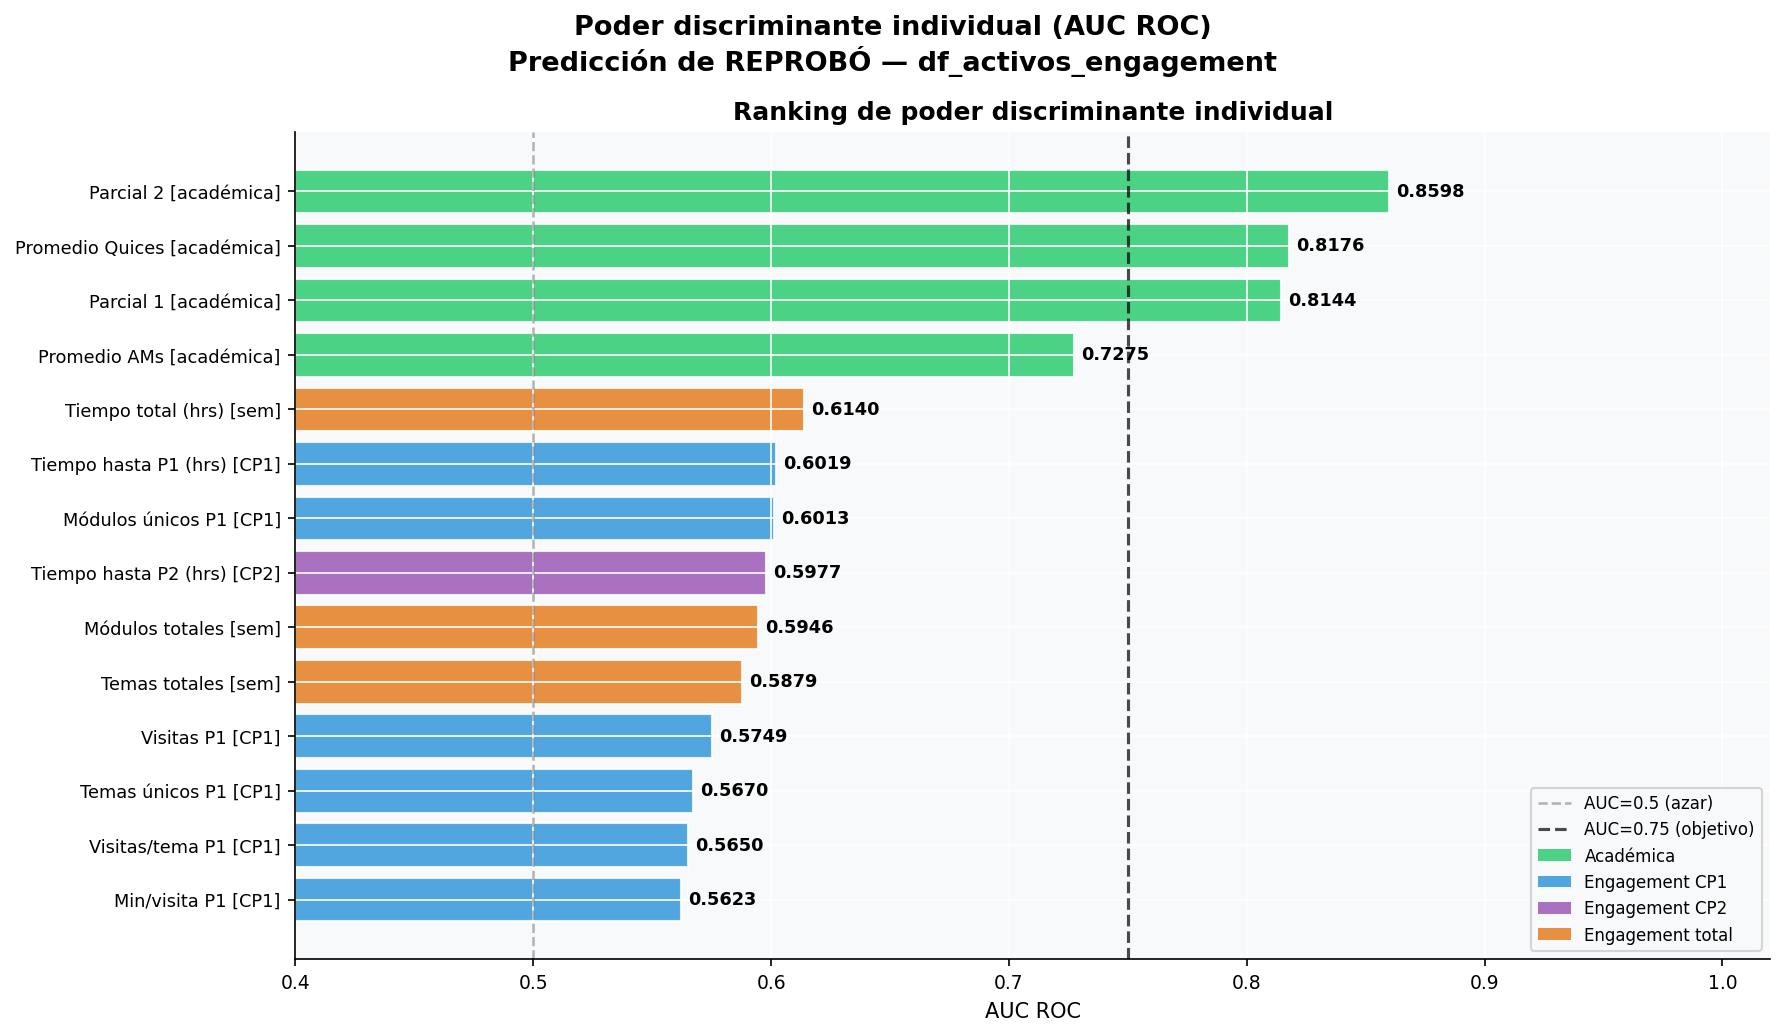
\includegraphics[width=0.92\textwidth]{06_auc_univariante_cp1.png}
  \caption{Poder discriminativo individual (AUC-ROC) de cada predictor candidato en CP1. Las variables académicas dominan la capacidad predictiva.}
  \label{fig:auc_univariante_cp1}
\end{figure}

Para cuantificar el aporte del engagement más allá de lo que ya captura P1, se calculó la correlación de Spearman entre el tiempo de engagement hasta P1 y la nota final, controlando por la nota de P1. El resultado es $\rho_\text{parcial} = 0{,}166$ ($p = 1{,}9 \times 10^{-4}$): el engagement explica un 2--3\,\% de varianza adicional en el resultado, modesto en términos absolutos pero estadísticamente robusto y operacionalmente relevante en la zona de incertidumbre del clasificador ($[2{,}5;\;3{,}5)$ en P1).

\FloatBarrier

\subsection{Multicolinealidad entre variables de engagement}

Las variables de engagement presentan correlaciones internas altas. Los pares más problemáticos son: tiempo hasta P1 $\leftrightarrow$ tiempo hasta P2 ($r = 0{,}864$), temas P1 $\leftrightarrow$ módulos P1 ($r = 0{,}861$) y temas total $\leftrightarrow$ módulos total ($r = 0{,}941$). Esta multicolinealidad justifica dos decisiones de diseño: aplicar regularización en los modelos lineales, e incluir en cada conjunto de características variables representativas de una sola dimensión (amplitud o profundidad, no ambas simultáneamente), en lugar de todas las variables de engagement de forma conjunta.

\section{Síntesis de decisiones de diseño}

El cuadro~\ref{tab:resumen_decisiones} sintetiza las decisiones de preprocesamiento y su justificación empírica. El conjunto de modelado resultante tiene tres características estructurales que condicionan la metodología del Capítulo~\ref{chap:metodologia}: desbalance de clases (74,3\,\% APROBÓ vs.\ 25,7\,\% REPROBÓ), que exige estrategias de balanceo; estructura longitudinal multisemestral, que invalida la validación cruzada aleatoria; y heterogeneidad pedagógica, que requiere variables de control por era.

\begin{table}[htbp]
  \centering
  \caption{Resumen de decisiones de diseño del conjunto de datos con justificación empírica e impacto cuantificado.}
  \label{tab:resumen_decisiones}
  \small
  \begin{tabular}{p{3.4cm}p{5.2cm}p{4.6cm}}
    \toprule
    Decisión & Justificación & Impacto \\
    \midrule
    Excluir RETIRADO y SIN NOTA
      & Etiqueta no observable; sesgo de retiro endógeno; heterogeneidad semántica
      & $N$: 764 $\to$ 554 \\[3pt]
    Excluir sin engagement
      & Cero ambiguo entre error y no-uso real
      & $N$: 554 $\to$ 502 \\[3pt]
    Excluir 3 variables de actividades
      & AUC-ROC $\leq 0{,}50$; $p > 0{,}05$
      & $-3$ predictores candidatos \\[3pt]
    Incluir \texttt{era\_encoded}
      & $\Delta$AUC-ROC(P1) = $-0{,}087$ entre eras
      & Control en todos los modelos \\[3pt]
    Incluir engagement
      & $\rho_\text{parcial} = 0{,}166$, $p < 0{,}001$
      & $+6$ predictores candidatos \\[3pt]
    Balanceo SMOTE / SMOTEENN
      & 74,3\,\% vs.\ 25,7\,\%; Recall sin balanceo $\approx 0{,}55$
      & Solo en training fold \\
    \bottomrule
  \end{tabular}
\end{table}

% ============================================================
%  CAPÍTULO 5 — METODOLOGÍA DE MODELADO
% ============================================================
\chapter{Metodología de Modelado}
\label{chap:metodologia}

Este capítulo describe la implementación técnica del SAT: los algoritmos evaluados, las métricas de evaluación, el manejo del desbalance, el esquema de validación y la construcción de variables.

\section{Algoritmos de clasificación evaluados}

Se evaluaron cuatro familias de algoritmos elegidas por su presencia dominante en la literatura de predicción académica \cite{Lopez2021} y su capacidad de manejar conjuntos de datos de tamaño moderado.

\subsection{Regresión Logística}

La Regresión Logística modela la probabilidad de la clase positiva mediante la función sigmoide aplicada a una combinación lineal de los predictores:
\begin{equation}
  P(y=1 \mid \mathbf{x}) =
  \frac{\exp(\beta_0 + \boldsymbol{\beta}^\top \mathbf{x})}
       {1 + \exp(\beta_0 + \boldsymbol{\beta}^\top \mathbf{x})},
\end{equation}
donde $\beta_0$ es el intercepto, $\boldsymbol{\beta} \in \mathbb{R}^p$ es el vector de 
coeficientes estimados por máxima verosimilitud, y $\mathbf{x}$ es el vector de 
características del estudiante. Los coeficientes tienen interpretación directa en términos de log-odds, es decir, el logaritmo de la razón entre la probabilidad de pertenecer a la clase positiva y la probabilidad de no pertenecer a ella:
\begin{equation}
\log\left(\frac{P(y=1 \mid \mathbf{x})}{1-P(y=1 \mid \mathbf{x})}\right)
= \beta_0 + \beta^\top \mathbf{x}.
\end{equation}
Esto facilita la explicación de las predicciones al docente~\cite{Lopez2021}. Para controlar el 
sobreajuste se aplica regularización L2 (Ridge, penaliza $\lambda\|\boldsymbol{\beta}\|_2^2$) 
o L1 (Lasso, penaliza $\lambda\|\boldsymbol{\beta}\|_1$, produce coeficientes nulos y hace 
selección implícita de variables)~\cite{Hastie2009}. El hiperparámetro $C = 1/\lambda$ controla 
la intensidad: valores pequeños de $C$ implican mayor regularización.

\subsection{Árbol de Decisión}

Un Árbol de Decisión particiona recursivamente el espacio de características mediante reglas binarias \cite{Breiman1984CART}. En cada nodo se selecciona el atributo $x_j$ y el umbral $t$ que minimizan la impureza de Gini en las ramas resultantes:
\begin{equation}
  G(S) = \sum_{k \in \mathcal{Y}} \hat{p}_k (1 - \hat{p}_k),
\end{equation}
donde $\hat{p}_k$ es la proporción de instancias de clase $k$ en el nodo $S$, y $\mathcal{Y} = \{0,1\}$ es el espacio de etiquetas. Los hiperparámetros de poda (máxima profundidad \texttt{max\_depth}, mínimo de muestras por hoja \texttt{min\_samples\_leaf}) controlan el equilibrio sesgo-varianza. Dado el tamaño moderado del conjunto de datos, se privilegió la poda agresiva para reducir sobreajuste.

\subsection{Random Forest}

El Random Forest (bosque aleatorio) combina $B$ árboles de decisión entrenados cada uno sobre una muestra bootstrap del conjunto de entrenamiento \cite{Breiman2001}. Una muestra bootstrap es una muestra aleatoria con reemplazo del mismo tamaño que el conjunto original. En cada nodo de cada árbol, solo un subconjunto aleatorio de $m \approx \sqrt{p}$ variables es candidato para la partición. La predicción final se obtiene por votación mayoritaria:
\begin{equation}
  \hat{y} = \arg\max_{k} \sum_{b=1}^{B} \mathbf{1}[h_b(\mathbf{x}) = k],
\end{equation}
donde $h_b(\mathbf{x})$ es la predicción del árbol $b$ para la observación $\mathbf{x}$. La combinación de múltiples árboles (ensamble) reduce la varianza sin aumentar el sesgo, produciendo modelos más estables que un árbol individual \cite{Breiman2001}.

\subsection{XGBoost}

XGBoost (Extreme Gradient Boosting) construye los árboles de manera secuencial: cada nuevo árbol $f_t$ minimiza la función de pérdida residual de los árboles anteriores \cite{Chen2016}:
\begin{equation}
  \mathcal{L}^{(t)} =
    \sum_{i=1}^{n}
    \ell\!\left(y_i,\, \hat{y}_i^{(t-1)} + f_t(\mathbf{x}_i)\right)
    + \Omega(f_t),
\end{equation}
donde $\ell(\cdot)$ es la log-pérdida binaria, $\hat{y}_i^{(t-1)}$ es la predicción acumulada de los $t-1$ árboles anteriores, y $\Omega(f_t) = \gamma T + \frac{1}{2}\lambda\|\mathbf{w}\|^2$ penaliza la complejidad del árbol: $T$ es el número de hojas, $\mathbf{w}$ son los pesos (valores de predicción) de cada hoja, y $\gamma$, $\lambda$ son los parámetros de regularización. Entre las ventajas prácticas de XGBoost se cuentan el procesamiento paralelo, el manejo nativo de valores faltantes y la regularización incorporada \cite{Chen2016}.

\section{Métricas de evaluación}

Las métricas se derivan de la matriz de confusión (Cuadro~\ref{tab:confusion}), que organiza las predicciones en cuatro categorías: Verdaderos Positivos (VP: reprobados correctamente identificados), Falsos Negativos (FN: reprobados no detectados), Falsos Positivos (FP: alertas innecesarias) y Verdaderos Negativos (VN: aprobados correctamente clasificados).

\begin{table}[htbp]
  \centering
  \caption{Matriz de confusión para clasificación binaria en el SAT. Un FN es un estudiante en riesgo no detectado (el error más costoso); un FP es una alerta innecesaria.}
  \label{tab:confusion}
  \begin{tabular}{llcc}
    \toprule
    & & \multicolumn{2}{c}{Predicción} \\
    \cmidrule(l){3-4}
    & & REPROBÓ & APROBÓ \\
    \midrule
    \multirow{2}{*}{Real}
      & REPROBÓ & VP & FN \\
      & APROBÓ  & FP & VN \\
    \bottomrule
  \end{tabular}
\end{table}

El Recall mide la proporción de reprobados detectados correctamente: $\text{Recall} = \text{VP} / (\text{VP} + \text{FN})$. Es la métrica prioritaria, pues el costo de no detectar a un estudiante en riesgo supera el de generar una alerta falsa \cite{Lopez2021}. La Precisión mide qué proporción de las alertas generadas corresponden a reprobados reales: $\text{Precisión} = \text{VP} / (\text{VP} + \text{FP})$. El F1-Score es la media armónica de Recall y Precisión, calculada por clase y promediada con peso igual (macro). El AUC-ROC cuantifica la capacidad discriminativa del modelo en todos los umbrales posibles \cite{Fawcett2006}: AUC-ROC = 0,5 equivale a clasificación aleatoria; 1,0 a clasificación perfecta. Es el filtro previo en la selección de modelos.

\section{Validación y tratamiento del desbalance de clases}

El conjunto de modelado presenta un desbalance de aproximadamente 3:1 
(74,3\,\% APROBÓ vs.\ 25,7\,\% REPROBÓ). Los clasificadores entrenados 
directamente sobre datos desbalanceados tienden a maximizar la exactitud 
global prediciendo casi siempre la clase mayoritaria, produciendo Recall 
bajo para REPROBÓ~\cite{He2009}. Para corregir esto, se implementan tres 
configuraciones: sin balanceo (distribución original, sirve como 
referencia), SMOTE~\cite{Chawla2002} y SMOTEENN~\cite{Batista2004}.

SMOTE genera instancias sintéticas de la clase minoritaria por 
interpolación lineal entre vecinos más cercanos:
\begin{equation}
  \mathbf{x}_\text{new} = \mathbf{x}_i + \delta \cdot 
  (\mathbf{x}_{nn} - \mathbf{x}_i), \quad \delta \sim \mathcal{U}(0,1),
\end{equation}
donde $\mathbf{x}_{nn}$ es uno de los $k$ vecinos más cercanos de 
$\mathbf{x}_i$ en la clase minoritaria. El parámetro $k$ se ajusta 
dinámicamente en cada fold ($k = \min(4, N_\text{min} - 1)$). 
SMOTEENN combina SMOTE con la técnica de limpieza Edited Nearest 
Neighbours (ENN): tras generar las muestras sintéticas, ENN elimina 
toda observación cuya etiqueta difiera de la mayoría entre sus $k$ 
vecinos más cercanos, limpiando las regiones ambiguas en la frontera 
de decisión.

En cuanto a la validación, la validación cruzada estándar $k$-fold 
asume que los datos son intercambiables, supuesto que no se cumple 
con datos de múltiples semestres con condiciones pedagógicas distintas. 
Por ello, se adopta Leave-One-Semester-Out (LOSO): en cada fold, un 
semestre actúa como conjunto de prueba y los cuatro restantes como 
entrenamiento. El cuadro~\ref{tab:loso_folds} describe la configuración 
de los cinco folds.

Cabe destacar que el balanceo se aplica exclusivamente al conjunto de 
entrenamiento dentro de cada fold; el conjunto de prueba conserva 
siempre la distribución original del semestre correspondiente. El 
Fold~4 (semestre 202510) es el más exigente, con una tasa de 
reprobación en prueba del 39,1\,\%, muy superior a la media global 
(25,7\,\%), lo que genera las caídas de desempeño más pronunciadas 
para todos los modelos. Las métricas reportadas son siempre la media 
$\pm$ desviación estándar sobre los cinco folds: la media estima el 
desempeño esperado ante un semestre futuro; la desviación estándar 
estima la estabilidad.

\begin{table}[htbp]
  \centering
  \caption{Configuración de los cinco folds LOSO. El Fold~4 (semestre 
  202510) es el más exigente por su tasa de reprobación en prueba 
  (39,1\,\%), muy por encima de la media global (25,7\,\%). La 
  heterogeneidad entre folds justifica reportar métricas como media 
  $\pm$ desviación estándar.}
  \label{tab:loso_folds}
  \small
  \begin{tabular}{clcrrc}
    \toprule
    Fold & Semestre de prueba & Era & $N_\text{train}$ & $N_\text{test}$ 
    & \% Reprobó (prueba) \\
    \midrule
    1 & 202320 & Antigua & 398 & 107 & 17,8\,\% \\
    2 & 202410 & Antigua & 433 &  72 & 18,1\,\% \\
    3 & 202420 & Nueva   & 383 & 122 & 27,0\,\% \\
    4 & 202510 & Nueva   & 390 & 115 & 39,1\,\% \\
    5 & 202520 & Nueva   & 416 &  89 & 22,5\,\% \\
    \bottomrule
    \multicolumn{6}{l}{\footnotesize Media global del conjunto de 
    modelado: 25,7\,\%.} \\
  \end{tabular}
\end{table}

\section{Variables derivadas y conjuntos de características}

\subsection{Variables derivadas}

Además de las variables brutas del sistema académico y de Bloque Neón, se construyeron siete variables derivadas que capturan dimensiones no expresadas directamente por las mediciones originales. Todas respetan el principio de causalidad temporal: ninguna variable disponible solo en CP2 se usa en modelos de CP1. El cuadro~\ref{tab:features_derivadas} describe cada variable y su intuición práctica.

\begin{table}[htbp]
  \centering
  \caption{Variables derivadas construidas para el modelado. La columna CP indica el checkpoint mínimo en que la variable puede usarse sin filtración temporal.}
  \label{tab:features_derivadas}
  \small
  \begin{tabular}{llp{5.8cm}c}
    \toprule
    Variable & Fórmula & Intuición & CP \\
    \midrule
    \texttt{era\_encoded}
      & $\mathbb{1}[\text{era nueva}]$
      & Controla el cambio estructural de las eras pedagógicas
      & CP1 \\[6pt]
    \texttt{log\_eng\_p1}
      & $\ln(1 + \text{eng}_{P1})$
      & Captura rendimientos decrecientes: pasar de 0 a 5~h de estudio importa más que pasar de 40 a 45~h
      & CP1 \\[6pt]
    \texttt{log\_eng\_p2}
      & $\ln(1 + \text{eng}_{P2})$
      & Ídem para el segundo período
      & CP2 \\[6pt]
    \texttt{p1\_vs\_media}
      & $\dfrac{P1 - \mu_\text{sem}}{\sigma_\text{sem}}$
      & Posición relativa del estudiante dentro de su cohorte; controla la dificultad del semestre
      & CP1 \\[10pt]
    \texttt{delta\_p2\_p1}
      & $P2 - P1$
      & Tendencia académica: positivo indica mejora, negativo indica declive entre parciales
      & CP2 \\[6pt]
    \texttt{intensidad\_p1}
      & $\dfrac{\text{eng}_{P1} \times 60}{\text{visitas}_{P1}}$
      & Minutos promedio por visita; distingue estudio profundo de vistazos rápidos
      & CP1 \\[10pt]
    \texttt{ratio\_vt\_p1}
      & $\dfrac{\text{visitas}_{P1}}{\text{temas\_únicos}_{P1}}$
      & Revisitas promedio por tema; valores altos indican repaso del mismo contenido
      & CP1 \\
    \bottomrule
  \end{tabular}
\end{table}
\FloatBarrier
\subsection{Conjuntos de características}

Los conjuntos de características se diseñaron bajo tres principios: gradación progresiva (de mínimo a máximo número de variables), causalidad temporal (sin filtración de datos hacia el futuro) y no redundancia (sin variables perfectamente colineales). Los cuadros~\ref{tab:feature_sets_cp1} y \ref{tab:feature_sets_cp2} describen los conjuntos para CP1 y CP2 respectivamente. Los conjuntos marcados con asterisco se evaluaron también con SMOTE y SMOTEENN, resultando en 17 configuraciones para CP1 y 20 para CP2.

\begin{table}[htbp]
  \centering
  \caption{Conjuntos de características evaluados en CP1. Los marcados con * se evaluaron también con SMOTE y SMOTEENN. Cada conjunto agrega información respecto al anterior, desde el más simple (S01: solo P1) hasta el más completo (S11: P1 + posición relativa + cuatro métricas de engagement).}
  \label{tab:feature_sets_cp1}
  \small
  \begin{tabular}{clcp{7cm}}
    \toprule
    ID & Nombre & $p$ & Variables incluidas \\
    \midrule
    S01 & solo\_parcial     & 1 & \texttt{parcial\_1} \\
    S02 & parcial\_era      & 2 & S01 + \texttt{era\_encoded} \\
    S03 & parcial\_relativo & 3 & S02 + \texttt{p1\_vs\_media} \\
    S04 & eng\_total        & 3 & S02 + \texttt{engagement\_hasta\_p1} \\
    S05 & eng\_log          & 3 & S02 + \texttt{log\_eng\_p1} \\
    S06 & eng\_calidad      & 4 & S04 + \texttt{parcial\_1\_tiempo\_por\_visita} \\
    S07$^*$ & eng\_cobertura & 5 & S04 + \texttt{modulos\_unicos\_P1} + \texttt{visitas\_por\_tema\_P1} \\
    S08$^*$ & base\_est     & 6 & S07 + \texttt{p1\_vs\_media} \\
    S09 & eng\_completo     & 7 & S08 + \texttt{parcial\_1\_tiempo\_por\_visita} \\
    S10 & derivadas         & 6 & \texttt{parcial\_1} + \texttt{p1\_vs\_media} + \texttt{log\_eng\_p1} + \texttt{intensidad\_p1} + \texttt{ratio\_vt\_p1} + \texttt{era\_encoded} \\
    S11$^*$ & completo      & 7 & S10 + \texttt{modulos\_unicos\_P1} \\
    \bottomrule
    \multicolumn{4}{l}{\footnotesize $p$: número de características. La variable \texttt{parcial\_1\_tiempo\_hrs} se excluyó de todos los conjuntos} \\
    \multicolumn{4}{l}{\footnotesize por colinealidad perfecta con \texttt{engagement\_hasta\_p1} ($r = 1{,}0$).} \\
  \end{tabular}
\end{table}

\begin{table}[htbp]
  \centering
  \caption{Conjuntos de características evaluados en CP2. Los marcados con * se evaluaron también con SMOTE y SMOTEENN. CP2 incorpora las calificaciones del segundo parcial, las evaluaciones continuas y el engagement acumulado hasta P2.}
  \label{tab:feature_sets_cp2}
  \small
  \begin{tabular}{clcp{7cm}}
    \toprule
    ID & Nombre & $p$ & Variables incluidas \\
    \midrule
    S01 & dos\_parciales      &  3 & \texttt{parcial\_1}, \texttt{parcial\_2}, \texttt{era\_encoded} \\
    S02 & ams                 &  4 & S01 + \texttt{promedio\_ams} \\
    S03 & academico           &  5 & S02 + \texttt{promedio\_quices} \\
    S04 & tendencia           &  3 & \texttt{parcial\_2}, \texttt{delta\_p2\_p1}, \texttt{era\_encoded} \\
    S05$^*$ & acad\_tendencia &  5 & S03 + \texttt{delta\_p2\_p1} (reemplaza \texttt{parcial\_1}) \\
    S06 & eng\_p1             &  5 & S01 + \texttt{engagement\_hasta\_p1} + \texttt{modulos\_unicos\_P1} \\
    S07$^*$ & base\_est\_cp2  & 10 & S03 + métricas detalladas de engagement P1 \\
    S08 & eng\_evol           &  4 & S01 + \texttt{log\_eng\_p1} + \texttt{log\_eng\_p2} \\
    S09 & eng\_p2\_det        &  8 & S01 + métricas detalladas de engagement P2 \\
    S10 & eng\_ambos          &  8 & S01 + métricas de engagement P1 y P2 \\
    S11$^*$ & tendencia\_deriv &  8 & S04 + \texttt{p1\_vs\_media} + \texttt{log\_eng\_p1} + derivadas \\
    S12$^*$ & completo\_cp2   & 12 & Combinación de todos los grupos anteriores \\
    \bottomrule
  \end{tabular}
\end{table}

% ============================================================
%  CAPÍTULO 6 — RESULTADOS
% ============================================================
\chapter{Resultados}
\label{chap:resultados}

Este capítulo presenta los resultados de la evaluación sistemática de 148 configuraciones (68 en CP1, 80 en CP2). Se presentan primero los resultados por algoritmo, luego los modelos finales seleccionados y finalmente la comparación entre checkpoints.

\section{Resultados en CP1 --- Checkpoint Semana~6}

Para CP1 se evaluaron 68 configuraciones. Todas superaron el umbral mínimo de AUC-ROC $\geq 0{,}75$, confirmando que la información de la semana~6 es suficiente para discriminar con relevancia entre grupos. Los cuadros~\ref{tab:cp1_lr} a \ref{tab:cp1_xgb} presentan las cinco mejores configuraciones por F1-Score para cada algoritmo.

\begin{table}[!htbp]
  \centering
  \caption{Cinco mejores configuraciones por F1-Score --- Regresión Logística, CP1. S05 (tres variables: P1, log del engagement hasta P1, y era pedagógica) logra el mayor F1 y la mayor Precisión. La transformación logarítmica del engagement captura la distribución asimétrica del tiempo de estudio mejor que el valor bruto. Valores = media LOSO sobre 5 folds.}
  \label{tab:cp1_lr}
  \small
  \begin{tabular}{lcccccc}
    \toprule
    Conjunto de características & $p$ & Balanceo & AUC-ROC & Recall & Precisión & F1 \\
    \midrule
    S05 (eng\_log)      & 3 & Ninguno & 0,844 & 0,732 & 0,637 & 0,666 \\
    S06 (eng\_calidad)  & 4 & Ninguno & 0,840 & 0,750 & 0,608 & 0,664 \\
    S04 (eng\_total)    & 3 & Ninguno & 0,842 & 0,717 & 0,632 & 0,661 \\
    S02 (parcial\_era)  & 2 & Ninguno & 0,843 & 0,705 & 0,635 & 0,641 \\
    S01 (solo\_parcial) & 1 & Ninguno & 0,843 & 0,756 & 0,565 & 0,639 \\
    \bottomrule
  \end{tabular}
\end{table}

\begin{table}[!htbp]
  \centering
  \caption{Cinco mejores configuraciones por F1-Score --- Árbol de Decisión, CP1. El AUC-ROC inferior respecto a LR y RF refleja la mayor varianza del árbol ante cambios en la composición del entrenamiento. El balanceo con SMOTE o SMOTEENN mejora el Recall a costa de precisión.}
  \label{tab:cp1_dt}
  \small
  \begin{tabular}{lcccccc}
    \toprule
    Conjunto de características & $p$ & Balanceo & AUC-ROC & Recall & Precisión & F1 \\
    \midrule
    S01 (solo\_parcial) & 1 & Ninguno  & 0,827 & 0,751 & 0,539 & 0,624 \\
    S07                 & 5 & SMOTE    & 0,807 & 0,741 & 0,560 & 0,624 \\
    S07                 & 5 & SMOTEENN & 0,808 & 0,749 & 0,561 & 0,623 \\
    S11                 & 7 & SMOTEENN & 0,808 & 0,727 & 0,574 & 0,613 \\
    S05 (eng\_log)      & 3 & Ninguno  & 0,785 & 0,683 & 0,565 & 0,611 \\
    \bottomrule
  \end{tabular}
\end{table}

\begin{table}[!htbp]
  \centering
  \caption{Cinco mejores configuraciones por F1-Score --- Random Forest, CP1. RF es consistente entre configuraciones (AUC-ROC $\approx 0{,}83$ en todas). S11 con SMOTE sube el Recall a 0,774, lo que lo hace candidato para el perfil de Máximo Recall.}
  \label{tab:cp1_rf}
  \small
  \begin{tabular}{lcccccc}
    \toprule
    Conjunto de características & $p$ & Balanceo & AUC-ROC & Recall & Precisión & F1 \\
    \midrule
    S05 (eng\_log)     & 3 & Ninguno & 0,834 & 0,717 & 0,635 & 0,665 \\
    S04 (eng\_total)   & 3 & Ninguno & 0,834 & 0,717 & 0,635 & 0,665 \\
    S11                & 7 & SMOTE   & 0,833 & 0,774 & 0,591 & 0,661 \\
    S02 (parcial\_era) & 2 & Ninguno & 0,830 & 0,764 & 0,571 & 0,652 \\
    S10 (derivadas)    & 6 & Ninguno & 0,831 & 0,712 & 0,613 & 0,651 \\
    \bottomrule
  \end{tabular}
\end{table}

\begin{table}[!htbp]
  \centering
  \caption{Cinco mejores configuraciones por F1-Score --- XGBoost, CP1. XGBoost logra el mayor Recall global en CP1 (0,806 con S11 y SMOTEENN, reportado en Tabla~\ref{tab:cp1_master}). Por F1-Score, S07 (cinco características con cobertura de engagement) ofrece el mejor balance.}
  \label{tab:cp1_xgb}
  \small
  \begin{tabular}{lcccccc}
    \toprule
    Conjunto de características & $p$ & Balanceo & AUC-ROC & Recall & Precisión & F1 \\
    \midrule
    S07 (eng\_cobertura) & 5 & Ninguno  & 0,829 & 0,788 & 0,568 & 0,658 \\
    S04 (eng\_total)     & 3 & Ninguno  & 0,831 & 0,731 & 0,600 & 0,657 \\
    S05 (eng\_log)       & 3 & Ninguno  & 0,831 & 0,731 & 0,600 & 0,657 \\
    S08                  & 6 & SMOTEENN & 0,808 & 0,775 & 0,585 & 0,653 \\
    S11 (completo)       & 7 & Ninguno  & 0,826 & 0,754 & 0,590 & 0,653 \\
    \bottomrule
  \end{tabular}
\end{table}

\FloatBarrier

El cuadro~\ref{tab:cp1_master} presenta la selección de modelos por perfil en CP1, resultado de la búsqueda global sobre las 68 configuraciones. Un resultado notable es la convergencia de los perfiles de Precisión y Balance: ambos seleccionan la misma Regresión Logística con S05, porque ningún modelo más complejo logra superar simultáneamente la Precisión y el F1 de esta combinación de tres variables (\texttt{parcial\_1}, \texttt{log\_eng\_p1}, \texttt{era\_encoded}). El perfil de Máximo Recall requiere XGBoost con S11 y SMOTEENN, alcanzando Recall = 0,806 a costa de una Precisión de 0,519: aproximadamente una de cada dos alertas generadas sería una falsa alarma.

\begin{table}[!htbp]
  \centering
  \caption{Selección de modelos por perfil operativo --- CP1 (semana~6). Búsqueda global sobre 68 experimentos con AUC-ROC $\geq 0{,}75$. En CP1, los perfiles Máxima Precisión y Balance (F1) convergen en el mismo modelo. $\tau^*$: umbral óptimo de clasificación.}
  \label{tab:cp1_master}
  \small
  \makebox[\textwidth][c]{%
  \resizebox{0.98\textwidth}{!}{%
  \begin{tabular}{lllllccccc}
    \toprule
    Perfil & Algoritmo & Conjunto & Bal. & $p$ & AUC-ROC & Recall & Precisión & F1 & $\tau^*$ \\
    \midrule
    Máx. Recall    & XGBoost & S11 & SMOTEENN & 7
      & $0{,}814_{\pm0.073}$ & $0{,}806_{\pm0.133}$ & 0,519 & $0{,}613_{\pm0.057}$ & 0,68 \\
    Máx. Precisión & LR & S05 & Ninguno & 3
      & $0{,}844_{\pm0.068}$ & $0{,}732_{\pm0.161}$ & $0{,}637$ & $0{,}666_{\pm0.024}$ & 0,35 \\
    Balance (F1)   & LR & S05 & Ninguno & 3
      & $0{,}844_{\pm0.068}$ & $0{,}732_{\pm0.161}$ & $0{,}637$ & $0{,}666_{\pm0.024}$ & 0,35 \\
    \bottomrule
    \multicolumn{10}{l}{\footnotesize En CP1, Máxima Precisión y Balance (F1) convergen en el mismo modelo (LR, S05, sin balanceo).} \\
  \end{tabular}
  }
  }
\end{table}

\FloatBarrier

La Figura~\ref{fig:metricas_cp1} presenta una comparación visual de las métricas AUC-ROC, Recall, Precisión y F1-Score para todos los algoritmos evaluados en CP1. Regresión Logística y Random Forest muestran el desempeño más equilibrado, con AUC-ROC superior a 0,84 y F1-Score cercanos a 0,64. XGBoost destaca en Recall (0,75) pero con una precisión más baja (0,57), lo que explica su selección para el perfil de Máximo Recall. El Árbol de Decisión presenta la mayor variabilidad y menores valores absolutos de AUC-ROC (0,79), reflejando su menor robustez en esta fase temprana del semestre.

\begin{figure}[!htbp]
  \centering
  
\includegraphics[width=0.92\textwidth]{fig_metricas_comparacion_cp1_profesional.png}
  \caption{Métricas de desempeño por algoritmo en CP1 (Semana 6). Promedios y desviaciones estándar sobre todas las configuraciones evaluadas ($n=68$). De izquierda a derecha: AUC-ROC, Recall, Precisión y F1-Score. LR (Regresión Logística) y RF (Random Forest) demuestran el mejor balance entre sensibilidad y especificidad, mientras que XGBoost prioriza la capacidad de detección (Recall) con trade-off en precisión.}
  \label{fig:metricas_cp1}
\end{figure}

\FloatBarrier

\section{Resultados en CP2 --- Checkpoint Semana~11}

Para CP2 se evaluaron 80 configuraciones. La incorporación del segundo parcial, las evaluaciones continuas y el engagement acumulado produce una mejora sustancial en todas las métricas respecto a CP1. La Tabla~\ref{tab:cp2_top5} presenta el top-5 global por F1-Score: la Regresión Logística con el conjunto académico-tendencia (S05 con SMOTE) domina, alcanzando AUC-ROC = 0,968 y F1 = 0,848.

\begin{table}[!htbp]
  \centering
  \caption{Cinco mejores configuraciones globales por F1-Score en CP2 (80 experimentos, AUC-ROC $\geq 0{,}75$). La Regresión Logística con el conjunto académico-tendencia (S05 + SMOTE) domina. Los AUC-ROC en CP2 ($> 0{,}95$) son sustancialmente mayores que en CP1 ($\approx 0{,}84$), reflejando el mayor poder discriminativo disponible en la semana~11.}
  \label{tab:cp2_top5}
  \small
  \makebox[\textwidth][c]{%
  \resizebox{0.98\textwidth}{!}{%
  \begin{tabular}{llccccc}
    \toprule
    Algoritmo & Conjunto de características & Balanceo & AUC-ROC & Recall & Precisión & F1 \\
    \midrule
    Reg. Logística & S05 (acad.\ tend.) & SMOTE   & 0,968 & 0,886 & 0,818 & 0,848 \\
    Reg. Logística & S05 (acad.\ tend.) & Ninguno & 0,967 & 0,867 & 0,824 & 0,842 \\
    XGBoost        & S03 (academico)    & Ninguno & 0,963 & 0,887 & 0,813 & 0,843 \\
    Random Forest  & S03 (academico)    & Ninguno & 0,953 & 0,819 & 0,823 & 0,820 \\
    Reg. Logística & S03 (academico)    & Ninguno & 0,956 & 0,880 & 0,744 & 0,800 \\
    \bottomrule
    \multicolumn{7}{l}{\footnotesize S05\_acad\_tendencia incluye: \texttt{parcial\_2}, \texttt{delta\_p2\_p1}, \texttt{promedio\_ams}, \texttt{promedio\_quices}, \texttt{era\_encoded}.} \\
  \end{tabular}
  }
  }
\end{table}

\FloatBarrier

\subsection{Análisis de Recall en CP2}

El análisis de Recall (capacidad de identificar correctamente los casos positivos) revela diferencias estratégicas entre los algoritmos. La Tabla~\ref{tab:cp2_top_recall} presenta las cinco configuraciones con mayor Recall. El Árbol de Decisión con el conjunto completo S11 + SMOTEENN alcanza un Recall de 0,932, identificando prácticamente la totalidad de estudiantes en riesgo. Sin embargo, este desempeño se acompaña de una menor precisión (0,536), indicando que el modelo genera un elevado número de falsos positivos.

La Regresión Logística mantiene un mejor balance, con configuraciones que alcanzan Recall de 0,918 (S05 + SMOTEENN) y 0,893 (S12 + SMOTEENN) con precisiones superiores a 0,72. Esta característica la convierte en la opción preferida para aplicaciones donde minimizar los falsos negativos es crítico, tales como sistemas de alerta temprana enfocados en intervención preventiva.

\begin{table}[!htbp]
  \centering
  \caption{Cinco mejores configuraciones por Recall en CP2 (capacidad de detección de casos positivos). Los algoritmos basados en árboles (DT, RF) logran los mayores Recall, aunque con trade-off en precisión. Reg. Logística mantiene balance superior.}
  \label{tab:cp2_top_recall}
  \small
  \makebox[\textwidth][c]{%
  \resizebox{0.95\textwidth}{!}{%
  \begin{tabular}{llccccc}
    \toprule
    Algoritmo & Conjunto de características & Balanceo & AUC-ROC & Recall & Precisión & F1 \\
    \midrule
    Árbol de Decisión & S11 (completo) & SMOTEENN & 0,866 & 0,932 & 0,536 & 0,672 \\
    Random Forest & S11 (completo) & SMOTEENN & 0,904 & 0,926 & 0,626 & 0,745 \\
    Reg. Logística & S05 (acad.\ tend.) & SMOTEENN & 0,958 & 0,918 & 0,732 & 0,810 \\
    XGBoost & S11 (completo) & SMOTEENN & 0,907 & 0,904 & 0,590 & 0,708 \\
    Reg. Logística & S12 (completo) & SMOTEENN & 0,946 & 0,893 & 0,724 & 0,799 \\
    \bottomrule
  \end{tabular}
  }
  }
\end{table}

\FloatBarrier

\subsection{Análisis de Precisión en CP2}

El análisis de Precisión (proporción de predicciones positivas correctas) muestra que XGBoost y Regresión Logística dominan cuando se requiere mayor confianza en las predicciones. La Tabla~\ref{tab:cp2_top_precision} presenta las configuraciones con máxima precisión. XGBoost con variables de engagement evolucionado (S06\_eng\_p1) alcanza una precisión de 0,846, aunque con un Recall moderado de 0,705. En contraste, la Regresión Logística con conjuntos académicos (S05 con SMOTE y S05 sin balanceo) logra precisiones superiores a 0,82 manteniendo Recall superior a 0,86, demostrando el balance superior de este algoritmo.

La comparación entre Recall y Precisión evidencia un trade-off fundamental: los modelos orientados a máxima sensibilidad (Recall) sacrifican especificidad (Precisión), mientras que los orientados a máxima precisión reducen su capacidad de cobertura. La Regresión Logística mitiga este trade-off de manera más efectiva, posicionándola como la mejor opción para aplicaciones que requieren ambas propiedades.

\begin{table}[!htbp]
  \centering
  \caption{Cinco mejores configuraciones por Precisión en CP2 (confiabilidad de predicciones positivas). XGBoost alcanza máxima precisión absoluta (0,846), pero Reg. Logística mantiene mejor balance recall-precisión.}
  \label{tab:cp2_top_precision}
  \small
  \makebox[\textwidth][c]{%
  \resizebox{0.95\textwidth}{!}{%
  \begin{tabular}{llccccc}
    \toprule
    Algoritmo & Conjunto de características & Balanceo & AUC-ROC & Recall & Precisión & F1 \\
    \midrule
    XGBoost & S06 (eng.\ p1) & Ninguno & 0,911 & 0,705 & 0,846 & 0,764 \\
    Reg. Logística & S05 (acad.\ tend.) & Ninguno & 0,967 & 0,867 & 0,824 & 0,842 \\
    Random Forest & S03 (académico) & Ninguno & 0,953 & 0,819 & 0,823 & 0,820 \\
    Reg. Logística & S05 (acad.\ tend.) & SMOTE & 0,968 & 0,886 & 0,818 & 0,848 \\
    XGBoost & S03 (académico) & Ninguno & 0,963 & 0,887 & 0,813 & 0,843 \\
    \bottomrule
  \end{tabular}
  }
  }
\end{table}

\FloatBarrier

El cuadro~\ref{tab:cp2_master} presenta la selección de perfiles para CP2. A diferencia de CP1, en CP2 los tres perfiles seleccionan algoritmos distintos: el Árbol de Decisión para Máximo Recall (único que supera Recall = 0,93), XGBoost para Máxima Precisión, y Regresión Logística para Balance. Esto evidencia que la mayor información disponible en CP2 permite explotar estructuras distintas de los datos según el objetivo de optimización. En particular, el conjunto académico puro (S03 y S05, basados en parciales y evaluaciones continuas) explica la mayor parte de la capacidad predictiva en CP2, mientras que las variables de engagement tienen menor peso relativo comparado con CP1.

\begin{table}[!htbp]
  \centering
  \caption{Selección de modelos por perfil operativo --- CP2 (semana~11). Búsqueda global sobre 80 experimentos con AUC-ROC $\geq 0{,}75$. A diferencia de CP1, los tres perfiles seleccionan algoritmos distintos. $\tau^*$: umbral óptimo de clasificación.}
  \label{tab:cp2_master}
  \small
  \makebox[\textwidth][c]{%
  \resizebox{0.98\textwidth}{!}{%
  \begin{tabular}{lllllccccc}
    \toprule
    Perfil & Algoritmo & Conjunto & Bal. & $p$ & AUC-ROC & Recall & Precisión & F1 & $\tau^*$ \\
    \midrule
    Máx. Recall    & DT & S11 & SMOTEENN & 8
      & $0{,}866_{\pm0.030}$ & $0{,}932_{\pm0.083}$ & 0,536 & $0{,}672_{\pm0.083}$ & 0,34 \\
    Máx. Precisión & XGB & S06 & Ninguno & 5
      & $0{,}911_{\pm0.051}$ & $0{,}705_{\pm0.110}$ & $0{,}846$ & $0{,}715_{\pm0.065}$ & 0,72 \\
    Balance (F1)   & LR & S05 & SMOTE & 5
      & $0{,}968_{\pm0.015}$ & $0{,}886_{\pm0.025}$ & $0{,}818$ & $0{,}848_{\pm0.055}$ & 0,54 \\
    \bottomrule
  \end{tabular}
  }
  }
\end{table}

\FloatBarrier

\subsection{Estadísticas Agregadas por Algoritmo en CP2}

La Tabla~\ref{tab:cp2_agregado} sintetiza el desempeño promedio de cada algoritmo sobre todas sus configuraciones en CP2. La Regresión Logística destaca con los valores más altos en AUC-ROC (0,945) y Precisión (0,748), mientras que mantiene un Recall competitivo (0,854). El Árbol de Decisión alcanza el Recall más elevado (0,814 en promedio) pero con la menor precisión (0,655), confirmando su orientación hacia la sensibilidad sobre la especificidad.

\begin{table}[!htbp]
  \centering
  \caption{Estadísticas agregadas por algoritmo en CP2 (promedios sobre todas las configuraciones, $\mu \pm \sigma$). LR domina en equilibrio; DT maximiza Recall; XGB equilibra AUC y Precisión.}
  \label{tab:cp2_agregado}
  \small
  \makebox[\textwidth][c]{%
  \resizebox{0.90\textwidth}{!}{%
  \begin{tabular}{lcccc}
    \toprule
    Algoritmo & AUC-ROC & Recall & Precisión & F1-Score \\
    \midrule
    Árbol de Decisión & $0{,}882 \pm 0{,}029$ & $0{,}814 \pm 0{,}053$ & $0{,}656 \pm 0{,}046$ & $0{,}711 \pm 0{,}064$ \\
    Reg. Logística & $0{,}945 \pm 0{,}011$ & $0{,}854 \pm 0{,}040$ & $0{,}748 \pm 0{,}032$ & $0{,}792 \pm 0{,}048$ \\
    Random Forest & $0{,}928 \pm 0{,}015$ & $0{,}807 \pm 0{,}040$ & $0{,}746 \pm 0{,}043$ & $0{,}765 \pm 0{,}055$ \\
    XGBoost & $0{,}932 \pm 0{,}016$ & $0{,}829 \pm 0{,}048$ & $0{,}738 \pm 0{,}060$ & $0{,}769 \pm 0{,}052$ \\
    \bottomrule
  \end{tabular}
  }
  }
\end{table}

\FloatBarrier

La Figura~\ref{fig:metricas_cp2} visualiza el desempeño comparativo de los algoritmos en CP2. El contraste es notable respecto a CP1: Regresión Logística demuestra una superioridad clara en todas las métricas, con AUC-ROC de 0,945 y F1-Score de 0,792. XGBoost y Random Forest mantienen desempeños similares entre sí (AUC-ROC $\approx 0{,}93$), mientras que el Árbol de Decisión presenta la mayor dispersión en las métricas, reflejando su dependencia de la estructura específica del conjunto de características.

\begin{figure}[!htbp]
  \centering
  
\includegraphics[width=0.92\textwidth]{fig_metricas_comparacion_cp2_profesional.png}
  \caption{Métricas de desempeño por algoritmo en CP2 (Semana 11). Promedios y desviaciones estándar sobre todas las configuraciones evaluadas ($n=80$). De izquierda a derecha: AUC-ROC, Recall, Precisión y F1-Score. La disponibilidad del segundo parcial y evaluaciones continuas permite que Regresión Logística alcance AUC-ROC = 0,945 y mantenga un balance óptimo entre Recall (0,854) y Precisión (0,748). Los algoritmos basados en árboles muestran mayor variabilidad.}
  \label{fig:metricas_cp2}
\end{figure}

\FloatBarrier

\section{Comparación Temporal: CP1 vs CP2}

La Figura~\ref{fig:cp1_vs_cp2} presenta un análisis comparativo del desempeño entre ambos checkpoints. El incremento en todas las métricas es sustancial: el AUC-ROC promedio mejora de 0,818 (CP1) a 0,922 (CP2), un aumento del 12,7\,\%. El F1-Score promedio sube de 0,631 (CP1) a 0,774 (CP2), una mejora del 22,6\,\%. Este progreso es impulsado principalmente por la disponibilidad del segundo parcial, que concentra aproximadamente el 18\,\% de la capacidad predictiva total en CP2, complementado por el aporte incremental de las evaluaciones continuas (aproximadamente 4--6\,\% adicional).

\begin{figure}[!htbp]
  \centering
  
\includegraphics[width=0.92\textwidth]{fig_metricas_comparacion_cp1_vs_cp2.png}
  \caption{Comparación de desempeño: CP1 (Semana 6, barras azules) vs CP2 (Semana 11, barras rojas). Cada métrica muestra promedios y desviaciones estándar. La información adicional disponible en CP2 (segundo parcial, evaluaciones continuas acumuladas) produce mejoras sustanciales: AUC-ROC aumenta 12,7\,\%, Recall 17,4\,\%, Precisión 22,7\,\% y F1-Score 22,6\,\% en promedio. Regresión Logística es el único algoritmo que mantiene desempeño más equilibrado en ambas fases.}
  \label{fig:cp1_vs_cp2}
\end{figure}

\FloatBarrier

En resumen, CP2 muestra mejoras sustanciales en todas las métricas respecto a CP1. El AUC-ROC promedio alcanza 0,922 (vs.\ 0,818 en CP1) y el F1-Score promedio es 0,774 (vs.\ 0,631 en CP1). La disponibilidad de información académica más completa (segundo parcial, evaluaciones continuas) es el factor determinante de estas mejoras, mientras que el engagement tiene menor poder predictivo relativo en esta fase más avanzada del semestre. La selección de perfiles diferenciados (Máximo Recall con DT, Máxima Precisión con XGB, Balance con LR) refleja la capacidad del conjunto de datos en CP2 para soportar múltiples objetivos operativos sin degradación severa de desempeño.

\section{Importancia de variables}

La Figura~\ref{fig:importancia_combinada} presenta la importancia por permutación ($\Delta$AUC-ROC) para Random Forest y XGBoost en CP1 y CP2. La importancia por permutación mide cuánto disminuye el AUC-ROC cuando los valores de una variable se permutan aleatoriamente; un $\Delta$AUC-ROC alto indica que el modelo depende fuertemente de esa variable.

En CP1, \texttt{parcial\_1} concentra $\Delta$AUC-ROC $\approx 0{,}32$--$0{,}36$, representando más del 85\,\% de la capacidad predictiva total. \texttt{engagement\_hasta\_p1} aporta $\Delta$AUC-ROC $\approx 0{,}05$--$0{,}06$ en RF y $\approx 0{,}005$ en XGB: contribución estadísticamente significativa pero sustancialmente menor que la nota del parcial. \texttt{era\_encoded} aporta consistentemente $\Delta$AUC-ROC $\approx 0{,}01$--$0{,}03$, validando su inclusión como variable de control.

En CP2, \texttt{parcial\_2} toma el liderazgo ($\Delta$AUC-ROC $\approx 0{,}18$), seguido de \texttt{parcial\_1} ($\approx 0{,}07$). Las evaluaciones continuas \texttt{promedio\_ams} y \texttt{promedio\_quices} aportan conjuntamente $\Delta$AUC-ROC $\approx 0{,}04$--$0{,}06$, capturando dimensiones del proceso de aprendizaje no completamente reflejadas en los parciales.

\begin{figure}[!htbp]
  \centering
  
\includegraphics[width=0.92\textwidth]{fig_importancia_combinada.png}
  \caption{Importancia de variables por permutación ($\Delta$AUC-ROC $\pm$ desviación estándar, 30 repeticiones) para Random Forest y XGBoost en CP1 y CP2. Solo se muestran variables con $\Delta$AUC-ROC~$> 0$. En CP1, \texttt{parcial\_1} concentra más del 85\,\% de la capacidad predictiva; el engagement aporta incrementalmente pero de forma secundaria. En CP2, \texttt{parcial\_2} toma el liderazgo y las evaluaciones continuas (AMs y quices) aportan un complemento significativo. Este patrón valida la estrategia de incorporar información de evaluación continua en modelos predictivos de riesgo académico.}
  \label{fig:importancia_combinada}
\end{figure}

\FloatBarrier

\section{Estabilidad y Robustez entre Semestres}

La robustez de un modelo predictivo depende no solo de su desempeño medio sino también de su consistencia entre semestres (folds LOSO). Un modelo con AUC medio alto pero desviación estándar elevada presenta riesgo de mal desempeño en semestres con composición atípica, reduciéndose su confiabilidad para producción.

En CP1, la Regresión Logística exhibe la menor varianza relativa en AUC-ROC ($\pm 0{,}068$), aunque el Recall muestra una desviación estándar considerable ($\pm 0{,}161$) por la heterogeneidad entre semestres. El Árbol de Decisión es el modelo menos estable globalmente, con desviaciones estándar promedio de $\pm 0{,}078$ en AUC-ROC y $\pm 0{,}129$ en Recall, indicando que sus reglas de decisión varían significativamente según el semestre de entrenamiento. XGBoost, aunque alcanza el mayor Recall medio (0,806), mantiene una desviación estándar de $\pm 0{,}133$, la mayor entre los modelos, lo que implica riesgo de mal desempeño en semestres con distribución atípica.

En CP2, todos los modelos mejoran sustancialmente su estabilidad gracias a la información adicional del segundo parcial. La Regresión Logística exhibe la menor varianza absoluta en AUC-ROC ($\pm 0{,}015$), posicionándose como el modelo más confiable para despliegue en producción. El Árbol de Decisión también mejora significativamente ($\pm 0{,}030$ en AUC-ROC), aunque mantiene una desviación estándar más alta en Recall ($\pm 0{,}083$) debido a su naturaleza sensible a cambios en la estructura de los datos. XGBoost y Random Forest convergen a desviaciones estándar similares en AUC-ROC ($\approx \pm 0{,}037$--$0{,}051$), manteniendo un balance razonable entre desempeño y variabilidad.

El patrón de mejora en estabilidad de CP1 a CP2 refuerza la conclusión de que la disponibilidad de información adicional (segundo parcial, evaluaciones continuas) no solo mejora el desempeño absoluto sino también la consistencia del modelo entre semestres.

\FloatBarrier

\section{Modelos Finales y Estrategia Operacional}

La evaluación exhaustiva de 148 configuraciones (68 en CP1 y 80 en CP2) sobre cuatro algoritmos distintos permitió la selección de seis modelos finales, tres por checkpoint, optimizados para tres objetivos operacionales diferentes: máxima capacidad de detección (Recall), máxima confiabilidad en las alertas (Precisión), y mejor equilibrio entre ambas (F1-Score). La Tabla~\ref{tab:modelos_finales} consolida estos modelos, mientras que la Tabla~\ref{tab:modelos_features} detalla las variables de entrada específicas.

\begin{table}[!htbp]
  \centering
  \caption{Seis modelos finales seleccionados: tres perfiles operacionales por checkpoint. Búsqueda global entre todas las familias (LR, DT, RF, XGB) y conjuntos de características, con AUC-ROC $\geq 0{,}75$ como requisito previo. Métricas = media $\pm$ desviación estándar sobre 5 folds LOSO.}
  \label{tab:modelos_finales}
  \small
  \makebox[\textwidth][c]{%
  \resizebox{0.98\textwidth}{!}{%
  \begin{tabular}{lllcccccc}
    \toprule
    CP & Perfil & Algoritmo --- Conjunto & Bal. & $p$ & AUC-ROC & Recall & Precisión & $\tau^*$ \\
    \midrule
    \multirow{3}{*}{CP1}
      & Máx. Recall    & XGBoost --- S11 & SMOTEENN & 7 & $0{,}814_{\pm0.072}$ & $0{,}806_{\pm0.133}$ & 0,519 & 0,68 \\
      & Máx. Precisión & LR --- S05      & Ninguno  & 3 & $0{,}844_{\pm0.068}$ & $0{,}732_{\pm0.161}$ & $0{,}637$ & 0,35 \\
      & Balance (F1)   & LR --- S05      & Ninguno  & 3 & $0{,}844_{\pm0.068}$ & $0{,}732_{\pm0.161}$ & $0{,}637$ & 0,35 \\
    \midrule
    \multirow{3}{*}{CP2}
      & Máx. Recall    & DT --- S11      & SMOTEENN & 8 & $0{,}866_{\pm0.030}$ & $0{,}932_{\pm0.083}$ & 0,536 & 0,34 \\
      & Máx. Precisión & XGB --- S06     & Ninguno  & 5 & $0{,}911_{\pm0.051}$ & $0{,}705_{\pm0.110}$ & $0{,}846$ & 0,72 \\
      & Balance (F1)   & LR --- S05      & SMOTE    & 5 & $0{,}968_{\pm0.015}$ & $0{,}886_{\pm0.025}$ & $0{,}818$ & 0,54 \\
    \bottomrule
    \multicolumn{9}{l}{\footnotesize En CP1, Máx. Precisión y Balance convergen en el mismo modelo. $p$ = número de variables; Bal. = técnica de balanceo; $\tau^*$ = umbral óptimo.} \\
  \end{tabular}
  }
  }
\end{table}

\FloatBarrier

\subsection{Análisis por Perfil Operacional}

Perfil Máximo Recall (detección exhaustiva): En CP1, XGBoost con el conjunto completo S11 alcanza Recall = $0{,}806$, identificando aproximadamente ocho de cada diez estudiantes en riesgo. Sin embargo, el costo es una precisión baja ($0{,}519$), lo que implica que aproximadamente una de cada dos alertas es falsa. En CP2, el Árbol de Decisión amplía el Recall a $0{,}932$ (casi universal), pero mantiene una precisión igualmente baja ($0{,}536$). Este perfil es apropiado para instituciones con suficientes recursos para intervenir a todos los estudiantes alertados y donde el costo de no detectar un caso en riesgo supera el costo de intervenciones innecesarias.

Perfil Máxima Precisión (alertas de alta confianza): En CP1, la Regresión Logística con solo tres variables (\texttt{parcial\_1}, \texttt{log\_eng\_p1}, \texttt{era\_encoded}) logra una precisión de $0{,}637$, aceptable pero limitada. En CP2, XGBoost con variables de engagement detalladas alcanza una precisión de $0{,}846$, la más alta entre todos los modelos. Sin embargo, el Recall cae a $0{,}705$, dejando sin detectar aproximadamente tres de cada diez casos en riesgo. Este perfil conviene en contextos donde el recurso de intervención es escaso y se prefiere invertir solo en casos de muy alto riesgo.

Perfil Balance (F1-Score máximo): En CP1, la Regresión Logística con S05 (sin balanceo) ofrece un balance moderado: AUC-ROC = $0{,}844$, Recall = $0{,}732$, Precisión = $0{,}637$, F1 = $0{,}666$. En CP2, el mismo algoritmo con SMOTE logra mejoras sustanciales: AUC-ROC = $0{,}968$, Recall = $0{,}886$, Precisión = $0{,}818$, F1 = $0{,}848$. Este modelo es el más versátil, recomendado como punto de partida para instituciones que no tienen preferencia clara entre maximizar detección o confiabilidad.

\begin{table}[!htbp]
  \centering
  \caption{Variables de entrada de cada modelo final. Las variables derivadas se calculan automáticamente a partir de las variables brutas del sistema académico. S05, S06, S11 refieren a conjuntos de características previamente definidos.}
  \label{tab:modelos_features}
  \small
  \begin{tabular}{llp{9cm}}
    \toprule
    CP & Perfil & Variables de entrada \\
    \midrule
    \multirow{2}{*}{CP1}
      & Máx. Recall     & \texttt{parcial\_1}, \texttt{p1\_vs\_media}, \texttt{log\_eng\_p1}, \texttt{parcial\_1\_modulos\_unicos}, \texttt{intensidad\_p1}, \texttt{ratio\_vt\_p1}, \texttt{era\_encoded} \\[4pt]
      & Prec.\ / Balance & \texttt{parcial\_1}, \texttt{log\_eng\_p1}, \texttt{era\_encoded} \\
    \midrule
    \multirow{3}{*}{CP2}
      & Máx. Recall     & \texttt{parcial\_2}, \texttt{delta\_p2\_p1}, \texttt{p1\_vs\_media}, \texttt{log\_eng\_p1}, \texttt{parcial\_1\_modulos\_unicos}, \texttt{parcial\_1\_visitas\_por\_tema}, \texttt{parcial\_1\_tiempo\_por\_visita}, \texttt{era\_encoded} \\[4pt]
      & Máx. Precisión  & \texttt{parcial\_1}, \texttt{parcial\_2}, \texttt{engagement\_hasta\_p1}, \texttt{parcial\_1\_modulos\_unicos}, \texttt{era\_encoded} \\[4pt]
      & Balance (F1)    & \texttt{parcial\_2}, \texttt{delta\_p2\_p1}, \texttt{promedio\_ams}, \texttt{promedio\_quices}, \texttt{era\_encoded} \\
    \bottomrule
  \end{tabular}
\end{table}

\FloatBarrier

\subsection{Mejora Incremental CP1 a CP2 y Trade-offs Operacionales}

La Tabla~\ref{tab:mejora_incremental} cuantifica el progreso al pasar del primer al segundo checkpoint. Tomando como referencia el modelo de Balance (F1) en cada uno, el AUC-ROC mejora de 0,844 a 0,968 (+12,4 puntos porcentuales), el Recall de 0,732 a 0,886 (+15,4 pp), y la Precisión de 0,637 a 0,818 (+18,1 pp). El F1-Score global aumenta de 0,666 a 0,848 (+18,2 pp), confirmando la hipótesis de que el segundo parcial y las evaluaciones continuas capturan información crítica para la predicción.

\begin{table}[!htbp]
  \centering
  \caption{Mejora incremental CP1 $\to$ CP2 en el modelo de Balance (F1). Comparación del mismo algoritmo (LR con S05) en ambos checkpoints. La mejora es sustancial en todas las métricas, pero implica reducir la ventana de intervención de aproximadamente 11 semanas (desde semana 6) a aproximadamente 6 semanas (desde semana 11).}
  \label{tab:mejora_incremental}
  \small
  \begin{tabular}{lccc}
    \toprule
    Métrica & CP1 & CP2 & $\Delta$ \\
    \midrule
    AUC-ROC   & 0,844 & 0,968 & $+0{,}124$ \\
    Recall    & 0,732 & 0,886 & $+0{,}154$ \\
    Precisión & 0,637 & 0,818 & $+0{,}181$ \\
    F1-Score  & 0,666 & 0,848 & $+0{,}182$ \\
    Exactitud & 0,808 & 0,929 & $+0{,}121$ \\
    \bottomrule
    \multicolumn{4}{l}{\footnotesize Algoritmo: LR; Conjunto: S05 (CP1 sin balanceo, CP2 con SMOTE).} \\
  \end{tabular}
\end{table}

Sin embargo, la mejora de desempeño conlleva un trade-off crítico: la ventana de intervención se reduce de aproximadamente once semanas (desde la semana 6 hasta el final del semestre) a aproximadamente seis semanas (desde la semana 11 hasta el final). Una ventana más corta limita el tiempo disponible para implementar intervenciones pedagógicas, asesorías intensivas o cambios en la estrategia de estudio del estudiante.

La decisión de cuál checkpoint activar depende del contexto institucional específico. Instituciones con capacidad de intervención rápida y alta tasa de respuesta podrían beneficiarse de CP2, aceptando el menor tiempo pero ganando 18 puntos porcentuales en confiabilidad de predicción. Instituciones con intervenciones más lentas o con limitaciones de recursos podrían preferir CP1, aceptando menor precisión pero ganando cinco semanas adicionales para la acción. Una estrategia híbrida es factible: usar CP1 como alerta temprana indicativa y CP2 como confirmación para intervención definitiva, aprovechando la sinergia entre ambos checkpoints.

\FloatBarrier

% ================================================================
% CAPÍTULO 7: HERRAMIENTA WEB PARA DOCENTES
% ================================================================

\chapter{Herramienta Web para Docentes}
\label{cap:herramienta_web}

\section{Introducción}

Con el objetivo de facilitar la adopción y el uso operacional de los modelos de predicción entrenados, se desarrolló SAT (Sistema de Alerta Temprana) Uniandes, una plataforma web basada en Streamlit diseñada específicamente para docentes y coordinadores académicos. Esta herramienta democratiza el acceso a las alertas de riesgo académico, permitiendo que profesionales sin expertise en machine learning puedan entrenar modelos, generar predicciones y tomar decisiones informadas sobre intervenciones con estudiantes en riesgo.

La plataforma adopta un flujo de trabajo integrado en seis etapas secuenciales que guían al usuario desde la creación de un proyecto (curso o materia) hasta la exportación de reportes analíticos. El diseño ha priorizando la experiencia del usuario, la claridad de mensajes y la validación de datos en cada paso, con énfasis en reducir barreras técnicas.

\section{Arquitectura General}

SAT Uniandes está construido sobre una arquitectura modular que separa responsabilidades en capas funcionales:

\begin{itemize}
    \item \textbf{Capa de presentación (ui.py):} Interfaz web interactiva basada en Streamlit que gestiona seis páginas principales: Proyectos, Entrenamiento, Predicción, Dashboard, Modelos y Exportación.

    \item \textbf{Capa de datos (data.py, registry.py):} Persistencia de proyectos, checkpoints, modelos y predicciones mediante JSON estructurado. Registry.py actúa como ORM simplificado, definiendo dataclasses para ProjectRecord, CheckpointRecord, ModelRecord y PredictionRunRecord.

    \item \textbf{Capa de machine learning (training.py, inference.py, models.py):} Orquestación del entrenamiento (búsqueda de hiperparámetros, validación, selección de umbral), inferencia en datos nuevos y gestión del ciclo de vida del modelo.

    \item \textbf{Capa de visualizaciones (charts.py):} Renderizado de gráficas interactivas con Plotly, incluyendo curvas ROC, matrices de confusión, distribuciones de riesgo y análisis cohort.

    \item \textbf{Capa de exportación (exporters.py):} Generación de reportes en Excel y PDF con formato profesional para distribución a equipos académicos.
\end{itemize}

La estructura de directorios sigue un patrón jerárquico: \emph{Proyectos} contienen \emph{Checkpoints}, los cuales almacenan \emph{Modelos} entrenados y \emph{Predicciones} realizadas. Cada nivel mantiene metadatos en JSON para auditabilidad y reproducibilidad.

\section{Módulos de la Aplicación}

\subsection{Módulo 01: Proyectos}

El módulo Proyectos permite la gestión de entidades de nivel superior, donde cada proyecto representa un curso, materia o cohorte académica. Un docente puede crear múltiples proyectos sin restricción, por ejemplo, Cálculo Diferencial  y Cálculo Integral.
\begin{figure}
    \centering
    \includegraphics[width=1\linewidth]{proyectos.png}
    \caption{Vista de Proyectos}
    \label{fig:placeholder}
\end{figure}
\FloatBarrier

\textbf{Funcionalidades principales:}

\begin{itemize}
    \item Crear proyecto con nombre y descripción opcional.
    \item Ver listado de todos los proyectos con metadatos: número de checkpoints, cantidad total de modelos, fecha de creación.
    \item Seleccionar proyecto activo (indica contexto para las siguientes etapas).
    \item Visualizar detalles del proyecto activo incluyendo estructura de checkpoints y estado de los modelos.
\end{itemize}

El diseño permite a los docentes mantener una biblioteca de cursos con historial independiente de entrenamientos y predicciones por cada materia.

\subsection{Módulo 02: Entrenamiento (Flujo de 4 pasos)}

El flujo de entrenamiento es asistido mediante un stepper visual que guía al usuario en cuatro etapas claramente delimitadas.
\begin{figure}
    \centering
    \includegraphics[width=1\linewidth]{entrenam.png}
    \caption{Vista de entrenamiento}
    \label{fig:placeholder}
\end{figure}
\FloatBarrier

\subsubsection*{Paso 1: Crear/Seleccionar Checkpoint}

Un checkpoint representa un momento temporal en el semestre (p.ej., "Semana 6 — Post Parcial 1" o "Semana 11 — Post Parcial 2") en el cual se realizarán predicciones. El usuario puede:

\begin{itemize}
    \item Seleccionar un checkpoint existente dentro del proyecto activo, o
    \item Crear uno nuevo especificando un nombre y descripción que contextualize el momento académico.
\end{itemize}

\subsubsection*{Paso 2: Cargar Dataset Histórico}

El usuario sube un archivo CSV o Excel conteniendo el historial de estudiantes del checkpoint. La plataforma:

\begin{itemize}
    \item Lee y valida el formato del archivo.
    \item Muestra preview de columnas con tipos de datos, porcentaje de valores nulos y valores únicos.
    \item Mantiene el dataset en memoria de sesión para los pasos posteriores.
\end{itemize}

\subsubsection*{Paso 3: Asignar Variables}

El usuario mapea columnas del dataset a roles funcionales:

\begin{enumerate}
    \item \textbf{Identidad:} ID único del estudiante, nombre completo.
    \item \textbf{Target (variable objetivo):} Columna binaria (0 = aprobó, 1 = reprobó).
    \item \textbf{Features numéricas:} Notas, engagement, índices derivados.
    \item \textbf{Features categóricas:} Grupo, sección, modalidad.
\end{enumerate}

\subsubsection*{Paso 4: Entrenar Modelo}

El usuario configura parámetros de entrenamiento en dos secciones: básica y avanzada.

\textbf{Parámetros básicos:}

\begin{itemize}
    \item \textbf{Algoritmo:} LR (Regresión Logística), DT (Árbol de Decisión), RF (Random Forest), XGB (XGBoost).
    \item \textbf{Validación:} Holdout (división simple), K-Fold (validación cruzada), LOSO (Leave-One-Semester-Out para grupos de semestres).
    \item \textbf{Balanceo de clases:} none, SMOTE, SMOTEENN (para datasets desbalanceados).
    \item \textbf{Métrica objetivo:} f1 (recomendada), precision, recall, auc.
    \item \textbf{Hiperparámetros:} Búsqueda automática (recomendada) o valores fijos.
    \item \textbf{Iteraciones de búsqueda:} Número de combinaciones a explorar (4--20, default 8).
\end{itemize}

\textbf{Parámetros avanzados (JSON):} El usuario puede personalizar rangos de búsqueda o valores fijos para cada algoritmo editando un bloque JSON expandible.

Tras hacer clic en "Entrenar modelo", la plataforma:

\begin{enumerate}
    \item Valida la integridad del dataset y configuración.
    \item Ejecuta búsqueda de hiperparámetros según modo seleccionado.
    \item Calcula métricas de validación (AUC, Recall, Precision, F1).
    \item Selecciona umbral óptimo según métrica objetivo.
    \item Persiste el modelo y metadatos.
    \item Activa automáticamente el modelo entrenado.
\end{enumerate}

\FloatBarrier
\subsection{Módulo 03: Predicción}

Una vez entrenado un modelo, el usuario carga un nuevo dataset de estudiantes activos (sin variable objetivo) para generar predicciones de riesgo.

\begin{figure}[!ht] % El !ht obliga a intentar ponerlo "Aquí" o "Arriba" en ese orden de prioridad
    \centering
    \includegraphics[width=1\linewidth]{Prediccion.png}
    \caption{Vista de Predicción}
    \label{fig:placeholder}
\end{figure}

\FloatBarrier

El flujo:

\begin{enumerate}
    \item Selecciona modelo activo (modelo versión más reciente y activo para el checkpoint).
    \item Sube dataset con mismas columnas de features que entrenamiento.
    \item Valida columnas requeridas.
    \item Ejecuta inferencia.
\end{enumerate}

Por cada estudiante, la plataforma genera:

\begin{itemize}
    \item \textbf{Probabilidad:} Probabilidad de reprobación según el modelo (0.0 -- 1.0).
    \item \textbf{Alerta binaria:} 1 si probabilidad $\geq$ umbral, 0 en caso contrario.
    \item \textbf{Nivel de riesgo:} Categorización en BAJO (0.00--0.35), MEDIO (0.35--0.60), ALTO (0.60--1.00).
\end{itemize}

Los resultados se almacenan como "corrida de predicción" (PredictionRunRecord) para auditoría y acceso posterior desde el dashboard.

\subsection{Módulo 04: Dashboard}

El dashboard proporciona análisis visual y detallado de predicciones realizadas. 
Consta de dos vistas:

\subsubsection*{Vista Cohorte}
\begin{figure}
    \centering
    \includegraphics[width=1\linewidth]{cohorte.png}
    \caption{Vista del Dashboard por cohorte}
    \label{fig:placeholder}
\end{figure}

\FloatBarrier
Muestra métricas agregadas y gráficas:

\begin{itemize}
    \item Tarjetas KPI: Total estudiantes, cantidad en riesgo ALTO, MEDIO, BAJO.
    \item Gráfica de distribución de riesgo (gráfica de barras por categoría).
    \item Histograma de probabilidades.
    \item Tabla interactiva de estudiantes ordenada por probabilidad descendente (permite filtrado, búsqueda).
\end{itemize}

\subsubsection*{Vista Individual}
\begin{figure}
    \centering
    \includegraphics[width=1\linewidth]{Individual.png}
    \caption{Vista del Dashboard Individual}
    \label{fig:placeholder}
\end{figure}
\FloatBarrier
Permite inspeccionar el perfil detallado de un estudiante seleccionado:

\begin{itemize}
    \item Tarjeta con ID, nombre, probabilidad y nivel de riesgo prominentes.
    \item Gauge visual de probabilidad.
    \item Tabla de factores principales: variables que más impactan la predicción en dirección positiva o negativa.
    \item Gráfica de percentiles: posición del estudiante en la distribución de la cohorte en variables clave.
    \item Gráfica de importancia de features.
\end{itemize}

\subsection{Módulo 05: Modelos}

La página Modelos permite comparar y gestionar versiones entrenadas para un checkpoint específico.
\begin{figure}
    \centering
    \includegraphics[width=1\linewidth]{modelos.png}
    \caption{Vista de Modelos}
    \label{fig:placeholder}
\end{figure}
\FloatBarrier
\textbf{Funcionalidades:}

\begin{itemize}
    \item \textbf{Timeline visual:} Muestra todas las versiones entrenadas en orden chronológico inverso.
    \item \textbf{Indicadores:} AUC y F1 para cada versión, badge de ACTIVO/INACTIVO.
    \item \textbf{Selector:} Elige qué versión inspeccionar.
    \item \textbf{Tabs de inspección:}
    \begin{itemize}
        \item Resumen: Métricas de validación, decisiones del modelo.
        \item Configuración: Hiperparámetros finales, modo de búsqueda, dataset origen.
        \item Predicciones: Historial de corridas de predicción asociadas al modelo.
    \end{itemize}
    \item \textbf{Activar modelo:} Botón que promueve una versión a "activo" (usado por defecto en predicciones).
    \item \textbf{Comparación:} Gráfica de comparación de métricas vs. modelo activo actual.
\end{itemize}

\subsection{Módulo 06: Exportación}

Una vez completada una predicción, el usuario puede descargar resultados en dos formatos:

\begin{itemize}
    \item \textbf{Excel (.xlsx):} Tabla con columnas ID, Nombre, Probabilidad, Nivel de Riesgo, Alerta.
    \item \textbf{PDF:} Reporte estilizado con resumen ejecutivo (total estudiantes, distribución de riesgo) y tabla de datos.
\end{itemize}

Los reportes se guardan con referencia para auditoría en la corrida de predicción.
\begin{figure}
    \centering
    \includegraphics[width=1\linewidth]{exportacion.png}
    \caption{Vista de Exportación}
    \label{fig:placeholder}
\end{figure}
\FloatBarrier
% ================================================================
% CAPÍTULO 8: DISCUSIÓN Y CONCLUSIONES
% ================================================================

\chapter{Discusión y Conclusiones}
\label{chap:discusion}

\section{Síntesis del Sistema y Validación de Hallazgos}

El desarrollo de SAT Uniandes representa la transición de modelos teóricos de \textit{machine learning} hacia una plataforma operacional, intuitiva y modular. El sistema sintetiza el proceso analítico en un flujo que abarca desde el entrenamiento hasta la exportación de alertas, priorizando la validación continua y la transparencia de los resultados para el usuario no técnico.

Los hallazgos principales validan la viabilidad del sistema bajo cinco pilares fundamentales:

\begin{itemize}
    \item Desempeño sobre umbrales: El sistema supera los criterios de éxito en ambos \textit{checkpoints}. En CP2, el perfil de Balance alcanza un AUC-ROC de $0{,}968$ y un F1-Score de $0{,}848$. Incluso en CP1 (semana 6), con información mínima, el sistema ya opera por encima de los mínimos institucionales.
    \item Dominancia académica: Las calificaciones son la señal más informativa. En CP1, el \texttt{parcial\_1} concentra más del 85\% de la capacidad predictiva, seguido por el \texttt{parcial\_2} en CP2.
    \item Valor incremental del engagement: Aunque no es el factor dominante ($\rho = 0{,}166$), las métricas del LMS aportan entre 1 y 5 puntos adicionales de AUC-ROC. Su utilidad es crítica en la \textit{zona de incertidumbre} (notas entre $2{,}5$ y $3{,}5$), donde el comportamiento en plataforma ayuda a refinar la predicción.
    \item Estabilidad de la simplicidad: Los modelos basados en Regresión Logística con 3--5 variables demostraron ser los más estables ante la variabilidad entre semestres (desviación estándar de AUC-ROC $\pm 0{,}017$ en CP2), superando en confiabilidad a arquitecturas más complejas.
    \item Sensibilidad a la tasa de reprobación: Se identificó que semestres con tasas de reprobación atípicas (como el 202510 con 39,1\%) actúan como los \textit{folds} más exigentes, sugiriendo que el sistema requiere una recalibración si las condiciones históricas del curso cambian drásticamente.
\end{itemize}

\section{Discusión de Implicaciones Prácticas y Comparativa}

Los resultados obtenidos (AUC-ROC de $0{,}814$ en CP1 y $0{,}968$ en CP2) se sitúan en el rango superior de lo reportado en la literatura académica reciente, superando en precisión y \textit{recall} a implementaciones similares basadas exclusivamente en datos de LMS \cite{Macfadyen2010, Romero2020}. Un factor diferenciador es el uso de validación \textit{Leave-One-Semester-Out}, lo que garantiza resultados conservadores y realistas frente a cohortes futuras.

Para ilustrar el impacto operacional, la Tabla~\ref{tab:impacto_practico} presenta una simulación sobre un grupo típico de 120 estudiantes (donde históricamente 31 estarían en riesgo real).

\begin{table}[!ht]
  \centering
  \caption{Impacto práctico de los perfiles de CP1 sobre un grupo de 120 estudiantes (31 en riesgo). Los perfiles de Máxima Precisión y Balance convergen en el mismo modelo para este corte.}
  \label{tab:impacto_practico}
  \small
  \setlength{\tabcolsep}{4pt}
  \begin{tabularx}{\textwidth}{Xcccc}
    \toprule
    Perfil & Alertas & Verdaderas & Falsas & No detectados \\
    \midrule
    Máximo Recall & $\sim$48 & $\sim$25 & $\sim$23 & $\sim$6 \\ \addlinespace
    Máx. Precisión / Balance & $\sim$36 & $\sim$23 & $\sim$13 & $\sim$8 \\
    \bottomrule
  \end{tabularx}
\end{table}

\FloatBarrier

La elección entre estos perfiles no es un problema técnico, sino institucional. Si el recurso para la intervención es un correo masivo o taller opcional, el perfil de Máximo Recall es óptimo; si se trata de tutorías personalizadas con cupo limitado, el perfil de Balance asegura que el recurso se asigne a quienes tienen el riesgo más alto confirmado.

\section{Limitaciones y Perspectivas Futuras}

A pesar del éxito del sistema, existen límites metodológicos que deben ser considerados. El tamaño de la muestra ($N = 502$) genera varianza en las estimaciones temporales, y factores no observables, como cambios en el perfil del docente o la dificultad intrínseca de los temas por era, no son capturados totalmente por los modelos actuales. Asimismo, el sistema está diseñado para predecir el rendimiento académico y no la deserción, la cual responde a factores socioeconómicos externos a la plataforma.

Hacia el futuro, el SAT posee un alto potencial de escalabilidad. La integración de calificaciones de cursos prerrequisito (como Probabilidad y Estadística) podría habilitar predicciones incluso antes del primer parcial. Además, la modularidad de la herramienta web permite que esta metodología sea extendida a otros cursos críticos de la Universidad de los Andes, sentando las bases para una red institucional de analítica educativa.

\section{Conclusiones Finales}

Este trabajo culmina con la implementación exitosa de un Sistema de Alerta Temprana que convierte datos históricos en decisiones pedagógicas informadas. Se demostró que la información tiene valor predictivo desde la semana 6 del semestre, y que un modelo simplificado de tres variables ---nota de parcial, logaritmo del \textit{engagement} y era pedagógica--- es suficiente para operar con éxito.

SAT Uniandes no reemplaza el juicio del docente; lo potencia. Al ofrecer múltiples perfiles de riesgo, la plataforma reconoce que no existe un único equilibrio óptimo, permitiendo que la intervención se ajuste a los recursos disponibles. En este equilibrio entre el rigor del \textit{machine learning} y la flexibilidad de la práctica docente radica la capacidad del sistema para mejorar las tasas de aprobación y el acompañamiento estudiantil en cursos de alto riesgo.

\FloatBarrier

% ============================================================
%  REFERENCIAS
% ============================================================
\clearpage
\addcontentsline{toc}{chapter}{Referencias}

\begin{thebibliography}{19}

\bibitem{Lopez2021}
J.~López-Zambrano, J.~A. Lara~Torralbo, y C.~Romero,
``Early prediction of student learning performance through data
mining: A systematic review,''
\textit{Psicothema}, vol.~33, no.~3, pp.~456--465, 2021.
PDF libre: \url{https://www.psicothema.com/pdf/4692.pdf}

\bibitem{Benitez2024}
A.~F. Benítez~Amaya,
\textit{Academic performance prediction system based on machine learning}.
Universidad de los Andes, 2024.
\url{https://repositorio.uniandes.edu.co/entities/publication/e7f54ea9-5d40-4aea-b12f-05e871064df3}

\bibitem{Garcia2019}
N.~García~Duarte,
\textit{Tomando decisiones: predicción del desempeño académico en
aspirantes a la maestría en Economía de la Universidad de los Andes}.
Universidad de los Andes, 2019.
\url{https://repositorio.uniandes.edu.co/bitstreams/1d463375-6ac1-4f7c-beb4-c7a5470dd249/download}

\bibitem{RodriguezOrtiz2025}
M.~Á. Rodríguez-Ortiz, P.~C. Santana-Mancilla, y L.~E. Anido-Rifón,
``Machine learning and generative AI in learning analytics for
higher education: A systematic review of models, trends, and
challenges,''
\textit{Applied Sciences}, vol.~15, no.~15, p.~8679, 2025.
\url{https://doi.org/10.3390/app15158679}

\bibitem{Breiman1984CART}
L.~Breiman, J.~H. Friedman, R.~A. Olshen, y C.~J. Stone,
\textit{Classification and Regression Trees}.
Belmont, CA, USA: Wadsworth, 1984.

\bibitem{Hastie2009}
T.~Hastie, R.~Tibshirani, y J.~Friedman,
\textit{The Elements of Statistical Learning},
2.ª~ed. New York, NY, USA: Springer, 2009.
PDF libre: \url{https://hastie.su.domains/ElemStatLearn/}

\bibitem{Breiman2001}
L.~Breiman, ``Random forests,''
\textit{Machine Learning}, vol.~45, no.~1, pp.~5--32, 2001.
PDF libre: \url{https://www.stat.berkeley.edu/~breiman/randomforest2001.pdf}

\bibitem{Chen2016}
T.~Chen y C.~Guestrin, ``XGBoost: A scalable tree boosting system,''
en \textit{Proc. 22nd ACM SIGKDD Int. Conf. Knowledge Discovery and
Data Mining}, 2016, pp.~785--794.
\url{https://dl.acm.org/doi/10.1145/2939672.2939785}

\bibitem{He2009}
H.~He y E.~A. Garcia, ``Learning from imbalanced data,''
\textit{IEEE Trans. Knowl. Data Eng.}, vol.~21, no.~9,
pp.~1263--1284, sep.\ 2009.
\url{https://cs.utah.edu/~piyush/teaching/he_imbalanced.pdf}

\bibitem{Chawla2002}
N.~V. Chawla, K.~W. Bowyer, L.~O. Hall, y W.~P. Kegelmeyer,
``SMOTE: Synthetic minority over-sampling technique,''
\textit{J. Artif. Intell. Res.}, vol.~16, pp.~321--357, 2002.
\url{https://www.jair.org/index.php/jair/article/view/10302}

\bibitem{Batista2004}
G.~E.~A.~P.~A. Batista, R.~C. Prati, y M.~C. Monard,
``A study of the behavior of several methods for balancing
machine learning training data,''
\textit{ACM SIGKDD Explor. Newslett.}, vol.~6, no.~1,
pp.~20--29, 2004.
\url{https://dl.acm.org/doi/10.1145/1007730.1007735}

\bibitem{Fawcett2006}
T.~Fawcett, ``An introduction to ROC analysis,''
\textit{Pattern Recognit. Lett.}, vol.~27, no.~8,
pp.~861--874, 2006.
PDF libre: \url{https://people.inf.elte.hu/kiss/13dwhdm/roc.pdf}

\bibitem{Tinto1993}
V.~Tinto,
\textit{Leaving College: Rethinking the Causes and Cures of
Student Attrition}, 2.ª~ed.
Chicago, IL, USA: University of Chicago Press, 1993.

\bibitem{Kerby2014}
D.~S. Kerby,
``The simple difference formula: An approach to teaching
nonparametric correlation,''
\textit{Compr. Psychol.}, vol.~3, p.~11.IT.3.4.1, 2014.

\bibitem{Macfadyen2010}
L.~P. Macfadyen y S.~Dawson,
``Mining LMS data to develop an `early warning system' for educators:
A proof of concept,''
\textit{Comput. Educ.}, vol.~54, no.~2, pp.~588--599, 2010.
DOI: \url{https://doi.org/10.1016/j.compedu.2009.09.008}

\bibitem{Romero2020}
C.~Romero y S.~Ventura,
``Educational data mining and learning analytics: An updated survey,''
\textit{WIREs Data Min. Knowl. Discov.}, vol.~10, no.~3, p.~e1355, 2020.
DOI: \url{https://doi.org/10.1002/widm.1355}

\bibitem{Whitehill2017}
J.~Whitehill, K.~Mohan, D.~T. Seaton, Y.~Rosen y D.~Tingley,
``Delving deeper into MOOC student dropout prediction,''
\textit{arXiv preprint arXiv:1702.06404}, 2017.

\bibitem{Tempelaar2015}
D.~T. Tempelaar, B.~Rienties y B.~Giesbers,
``In search for the most informative data for feedback generation:
Learning analytics in a data-rich context,''
\textit{Comput. Human Behav.}, vol.~47, pp.~157--167, 2015.
DOI: \url{https://doi.org/10.1016/j.chb.2014.05.038}

\bibitem{Conijn2017}
R.~Conijn, C.~Snijders, A.~Kleingeld y U.~Matzat,
``Predicting student performance from LMS data: A comparison of
17 blended courses using Moodle LMS,''
\textit{IEEE Trans. Learn. Technol.}, vol.~10, no.~1, pp.~17--29, 2017.
DOI: \url{https://doi.org/10.1109/TLT.2016.2616312}

\end{thebibliography}

\end{document}
